\documentclass[preprint,12pt]{elsarticle}
\usepackage{graphicx}
\usepackage[margin=1.0in]{geometry}
\usepackage{color, colortbl}
\usepackage{hyperref}
\usepackage{float}
% \usepackage[affil-it]{authblk}
\usepackage{subcaption}
\newcommand{\note}[1]{\textcolor{blue}{#1}}
\definecolor{LightCyan}{rgb}{0.88,1,1}
\definecolor{LightRose}{rgb}{1,0.88,0.88}
\definecolor{LightGreen}{rgb}{0.88,1,0.88}

\title{CLAS12 Track Reconstruction With Artificial Intelligence }
\author[1]{Gagik Gavalian}
\author[2]{Polykarpos Thomadakis}
\author[2]{Angelos Angelopoulos}
\author[2]{Nikos Chrisochoides}
\author[3]{Raffaella De Vita}
\author[1]{Veronique Ziegler}

% \affiliation[1]{organization={CRTC, Department of Computer Science, Old Dominion University}, city={Norfolk, VA}, country={USA}}
\address[1]{Jefferson Lab, Newport News, VA, USA}
\address[2]{CRTC, Department of Computer Science, Old Dominion University, Norfolk, VA, USA}
\address[3]{INFN, Sezione di Genova, 16146 Genova, Italy}
%Authored by Jefferson Science Associates, LLC under U.S. DOE Contract No. DE-AC05-06OR23177. The U.S. Government retains a non-exclusive, paid-up, irrevocable, world-wide license to publish or reproduce this manuscript for U.S. Government purposes.
%\fntext[fn1]{Authors contributed equally.}
%\fntext[fn2]{Correspoding author, \textit{gavalian@jlab.org}}

\begin{document}

%\begin{titlepage}
\begin{abstract}

  In this article we describe the implementation of Artificial Intelligence models in track reconstruction software for the CLAS12 detector at Jefferson Lab.
 The Artificial Intelligence based approach resulted in improved track reconstruction efficiency in high luminosity experimental conditions.  The track
 reconstruction efficiency increased by $15\%$ for single particle, and statistics in multi-particle physics reactions increased by $15\%-35\%$ depending 
 on the number of particles in the reaction. The implementation of artificial intelligence in the workflow also resulted in code speedup of $35\%$.
\end{abstract}
%\end{titlepage}
\maketitle


\section{Introduction}
\indent

Nuclear Physics experiments have become increasingly complex over the past decades, using higher beam energies and higher beam currents. In emerging experiments where data collection rates are higher, there is a need for new approaches for data processing that can improve data reconstruction accuracy and speed. New developments in the Artificial Intelligence (AI) field present promising alternatives to conventional algorithms for data processing. Machine Learning (ML) algorithms are being employed in various stages of experimental data processing, such as: the detector data reconstruction, particle identification, detector simulations and physics data analysis. 

In this paper we present the implementation of previously developed machine learning models into the CLAS12 track reconstruction software. Detailed analysis 
of the reconstruction performance presented comparing track reconstruction efficiency and speed improvements to conventional algorithms.


\section{Particle Tracking}

The CLAS12\cite{Burkert:2020akg} detector is built around a six-coil toroidal magnet which divides the active detection into six azimuthal regions, called "sectors". Each sector is equipped with three regions of drift chambers. Each region consists of two chambers (caller super-layers), with each of them having 6 layers of wires. Each layer of wires in super-layer contains 112 wires making a super-layer a 6x112 wire matrix. The schematic view of one super-layer is shown on Figure~\ref{dc:side_view} (right panel).

\begin{figure}[!ht]
\begin{center}
 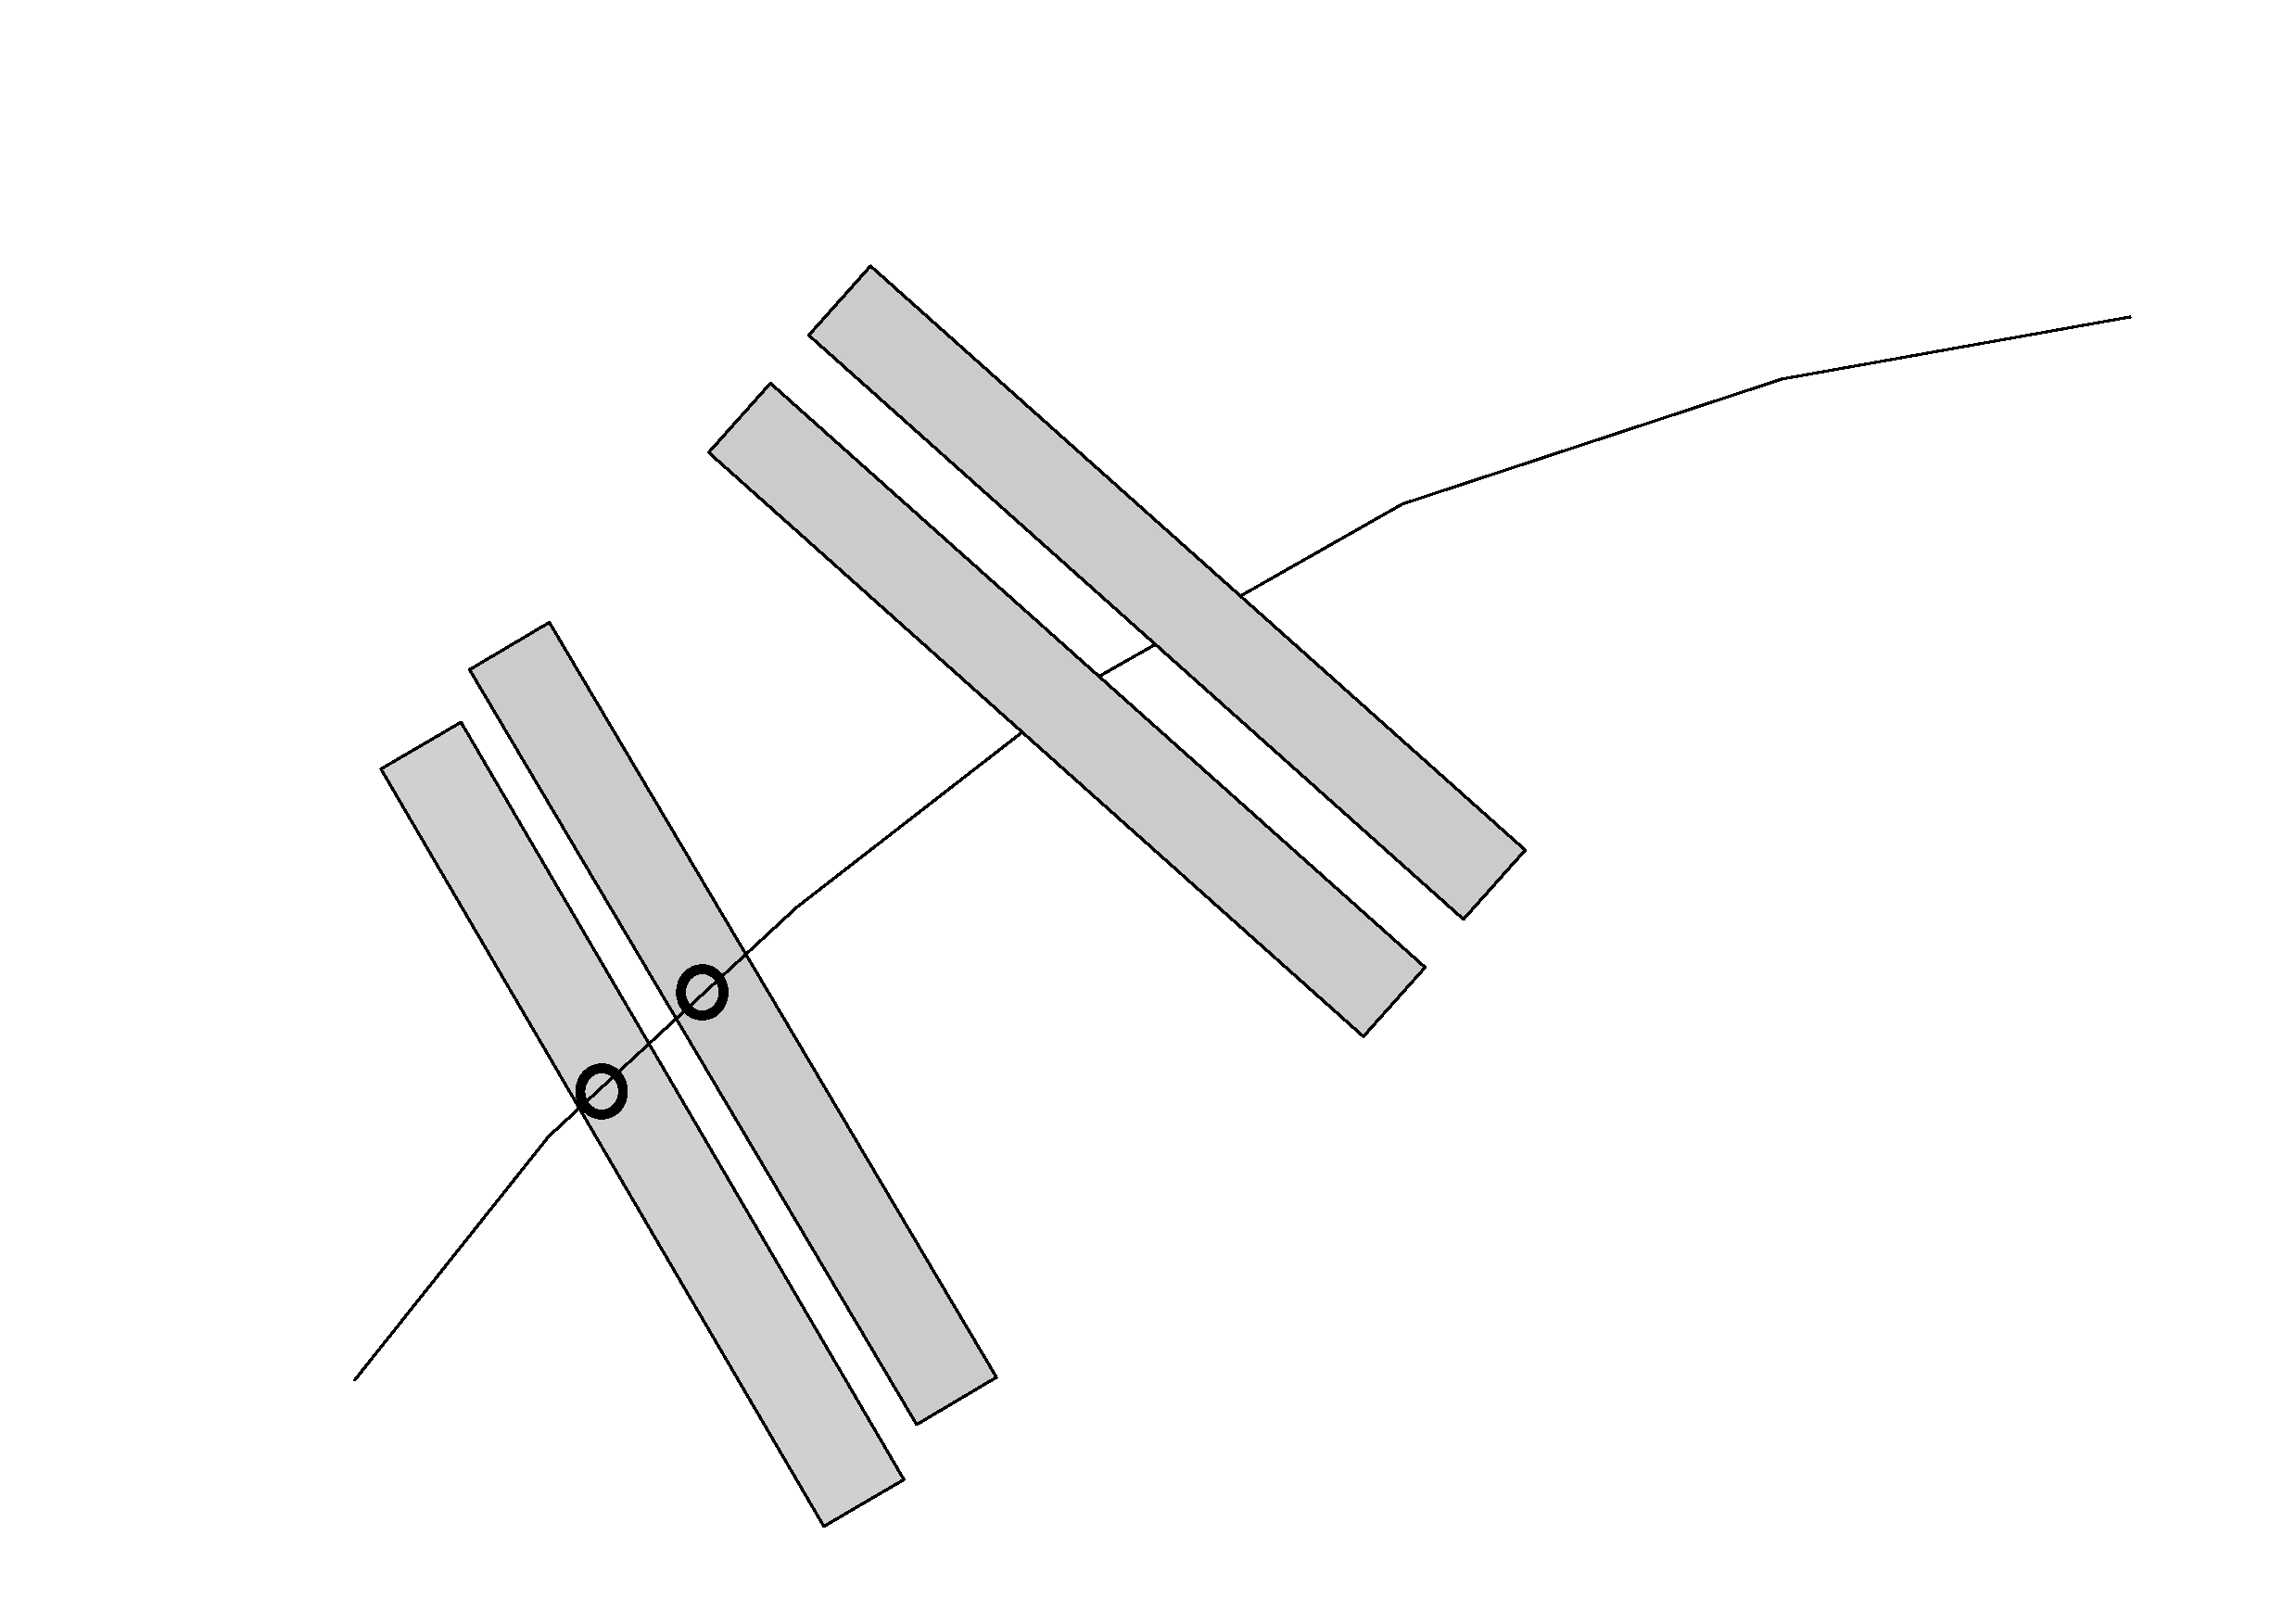
\includegraphics[width=3.5in]{images/dc_side_view.pdf}
 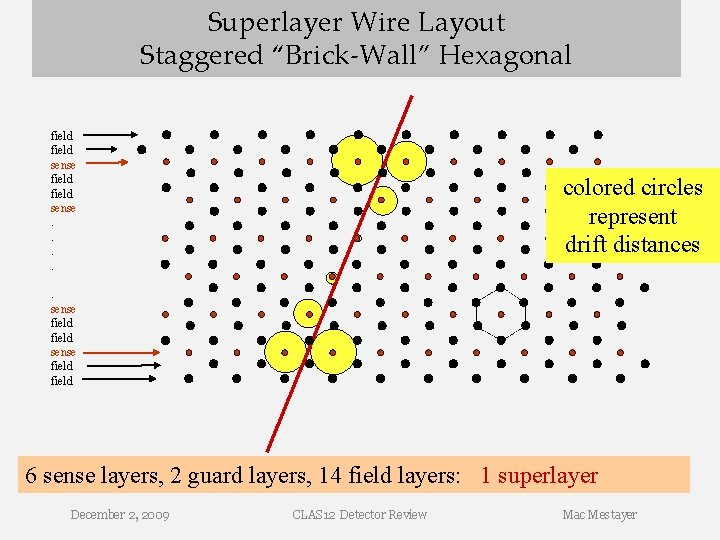
\includegraphics[width=2.5in]{images/image-29.jpg}
\caption {Side and front view of drift chambers. a) the layout for one sector showing three regions of drift chamber. Z-axis is direction of incoming beam. b) diagram of wire directions in each super layer.}
 \label{dc:side_view}
 \end{center}
\end{figure}

Particle that originates at interaction vertex in forward direction that pass through all three regions of the drift chamber in given sector are reconstructed by tracking algorithms. First adjacent  wires in each super-layer with a signal are grouped together into clusters (called segments), then track candidates are constructed by forming 6 segment combinations (one per each super-layer). Each track candidate is validated by tracking algorithm by performing a polynomial fit to determine if the candidate can be a real track. Once track candidates are isolated they are further refined using Kalman filter to measure particle parameters (such as momentum and angles). 
There are many experiments conducted with CLAS12 detector which have different running conditions (i.e. different targets and beam currents).
The changing beam energies and beam intensities (current) affect the amount of background that is detected in each detector components. For drift chambers the added background can be in a form of random hits that can be isolated by noise reducing algorithm, and can be in form of segments that do not belong to a track. With increased luminosity (beam current and target combination) number of combinatorics and the candidates to consider significantly increases, and this leads to decreased efficiency in track reconstruction. Recent studies done with experimental data and simulation showed that the tracking efficiency decreases with a rate of $0.44\%$ per nA of beam current. This leads to tracking efficiency at standard experimental running conditions (which is $45~nA$ electron beam incident on $40~cm$ liquid hydrogen target) is $\approx 80\%$.
The decrease of the efficiency of tracking what prevents experiments to run at higher beam currents (interaction rates), and increasing tracking efficiency will allow experiments to run for shorter time to collect desired statistics for physics results. 

\section{Machine Learning}

The Machine Learning approach was to teach the neural network to recognize good tracks
 from a large list of candidates. 
 Two neural networks were developed: a classifier network that can identify good track from  6 segment
 track candidates  and an auto-encoder that can take a list of 5 segment tracks and make them into 6 segment 
 track candidates by adding a pseudo-segment. The composed 6 super-layer track candidates (with pseudo-cluster)
 can be processed with classifier network to identify and isolate "good" track candidates.

 %The implementation consisted of two neural networks: a classifier network
 %that can identify good track from  6 segment track candidates  and a auto-encoder that can take a list of
 %5 segment tracks and make them into 6 segment track candidates by adding a pseudo-segment.
 
 \subsection{Track Classifier}
 
 To determine what type of architecture works best with CLAS12 drift chamber data we investigated different 
 types of neural network including Convolutional Neural Network (CNN) , Extremely Randomized Trees (ERT) and 
 Multi-Layer Perceptron (MLP) \cite{Gavalian:2020oxg}. The study showed that Multi-Layer Perceptron was best suited for 
 CLAS12 reconstruction needs (based on inference speed and accuracy). The implemented architecture is shown on 
 Figure~\ref{mlp:architecture}, where an input layer with 6 nodes is used (each node representing average wire position 
 of the segment in super-layer) and 3 output nodes for classes "positive track", " negative track" and "false track".
 
 \begin{figure}[!ht]
\begin{center}
 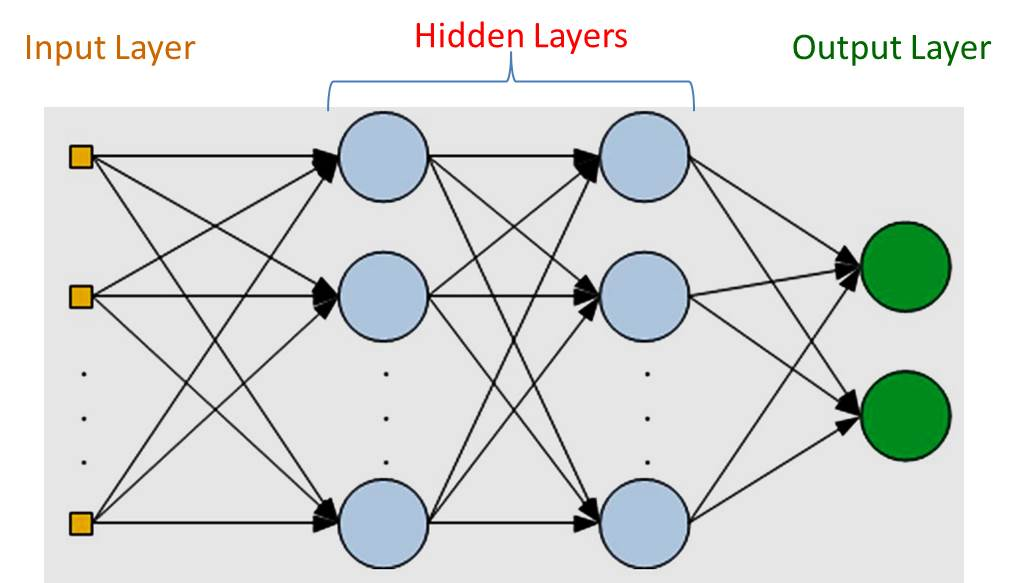
\includegraphics[width=3.5in]{images/Multilayer-Perceptron.jpg}
% 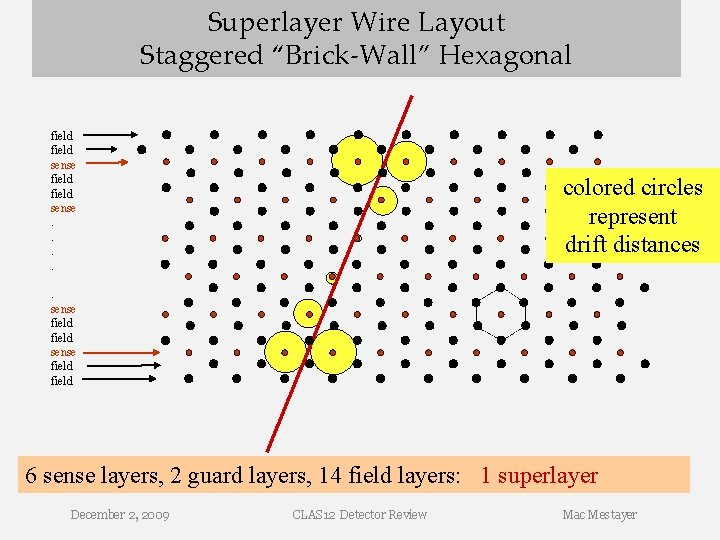
\includegraphics[width=2.5in]{images/image-29.jpg}
\caption {Architecture of Multi-Layer Preceptron.}
 \label{mlp:architecture}
 \end{center}
\end{figure}

The network is trained using results from processed data where the conventional algorithm has already 
identified good tracks (with a cut on $\chi^2$ to select very good quality tracks), which are fed to the network with
their respective labels (i.e. positive or negative tracks). For false tracks a combination of segments (6 segments 
forming a track candidate) is chosen that was not identified as a track by conventional algorithm.
 
 \subsection{Corruption Auto-Encoder}
 
The second neural network was developed to fix the corruption in possible track candidates due to 
inefficiencies of drift chambers. This network will be used to identify track candidates which have one of the segments
missing. We used auto-encoder type of neural network to implement feature fixing neural network \cite{Gavalian:2020xmc}. 
The structure of the network can be seen on Figure~\ref{autoencoder:architecture}, with 6 input nodes and six output nodes.

 \begin{figure}[!ht]
\begin{center}
 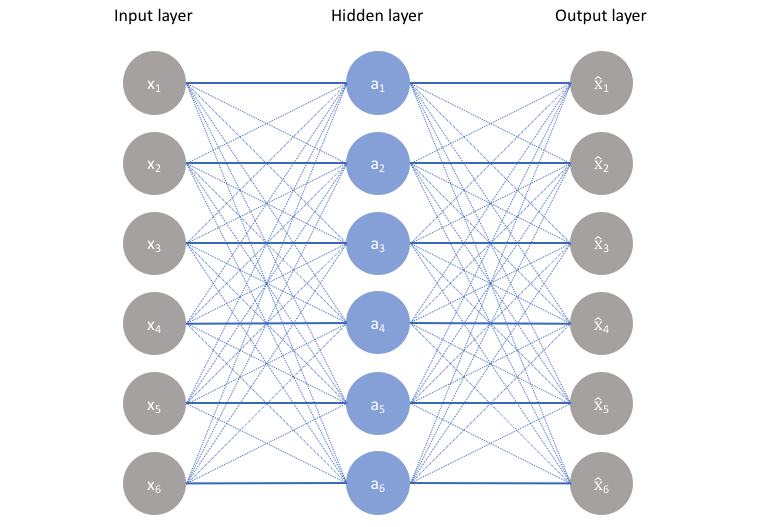
\includegraphics[width=2.0in]{images/auto_encoder.png}
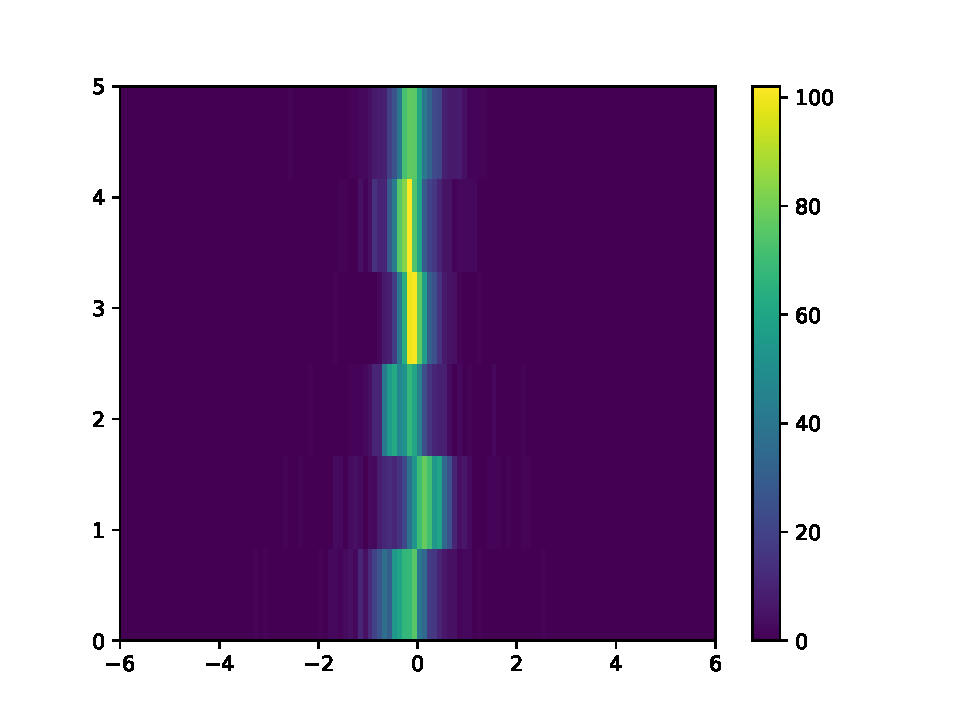
\includegraphics[width=2.0in]{images/auto_encoder_result_2d.pdf}
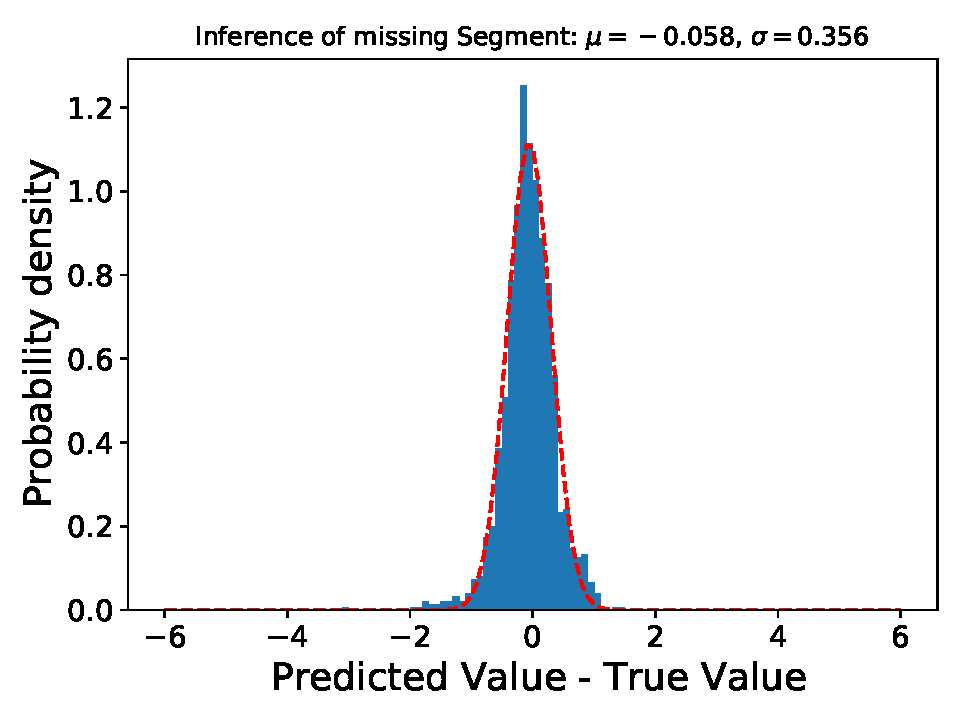
\includegraphics[width=2.0in]{images/auto_encoder_result_1d.pdf}
\caption {Architecture of corruption fixing Auto-Encoder.}
 \label{autoencoder:architecture}
 \end{center}
\end{figure}

To train the network good track candidates reconstructed by conventional tracking algorithm are used (same sample 
as for track classifier network training). The output for the network was set to the good track parameters (where all 6 
segments have non-zero values) and the input was modified by setting one of the nodes (randomly) to zero. The network
learns to fix the node containing zero by assigning it a value based on the other 5 segment values. The test results 
of the trained network are shown on Figure~\ref{autoencoder:architecture}, where the difference between true value 
of the segment position and reconstructed by network position is plotted, showing reconstruction accuracy of $0.36$ wires.
On Figure~\ref{autoencoder:architecture} this difference is shown vs the super-layer number which was corrupted in the input, 
as can be seen the performance of the network is uniform across all super-layers.

%\subsection{Implementation in reconstruction software}
%The CLAS12 track reconstruction software consist of several parts. The first stage of the process is to isolate clusters
%from the hits in drift chambers (called clustering service) . Once the clusters are isolated track candidates are formed from all combinations 
%of 6 segments. The track candidates are analyzed to determine which good candidates, from remaining segments 
%combinations of 5 segment tracks are constructed and these are also fitted to determine which ones are potential good tracks.
%The later module (hit based tracking) determines good track candidates based only on hit positions of the track candidates (no timing
%informations is used at this level). At the later stages of tracking code (time based tracking), chosen good track candidates are further refined by use of Kalman filter by using timing information from each of the sensors (drift chamber wires). By the time the reconstruction code reaches time based
%tracking stage the track candidates are already defined. 

%\begin{figure}[!ht]
%\begin{center}
% 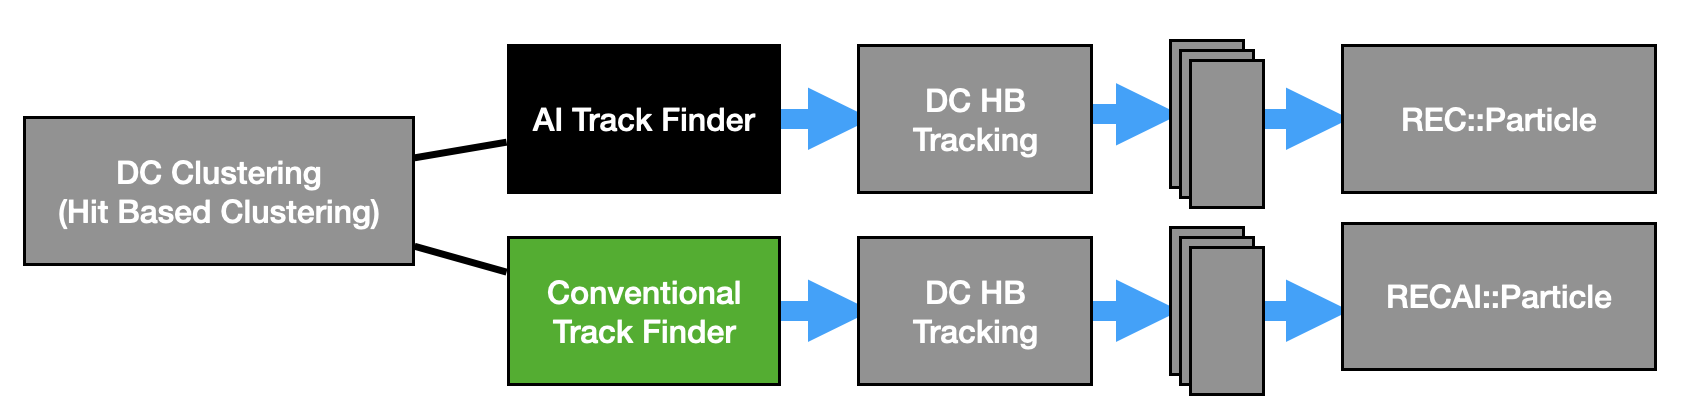
\includegraphics[width=6.0in]{images/recon_diagram.png}
%\caption {Architecture of corruption fixing Auto-Encoder.}
% \label{recon:diagram}
% \end{center}
%\end{figure}

%In order to implement our neural network into reconstruction workflow we designed two parallel branches in reconstruction code where we run 
%two algorithms to identify good tracks from track candidate lists, one based on conventional algorithm and second based on neural network.
%Both algorithms store their track suggestions in separate data structures, and pass them to the next stage where track parameters are reconstructed by 
%conventional tracking algorithm using Kalman filter. This approach let's us have two parallel outputs from tracking code in order to compare performance of
%each of the methods.


\section{Implementation of the Neural Network in CLAS12 software}

The models described in the previous sections were implemented in the CLAS12 tracking software. 

\subsection{Track Identification Workflow}

 Track identification consists of two phases, programmed to be done in two passes.
%First, all clusters reconstructed by the clustering algorithm are grouped into sectors and super-layers.
In the first pass over the data, signals from each sector of drift chambers are analyzed to create a track 
candidate list, each consisting of 6 segments.
The resulting track candidates are evaluated by the classifier neural network and are assigned a probability for 
being either positive or negative track. The list of track candidates is sorted by probability and passed
to another algorithm that is responsible for removing tracks that have lower probability of being a "good" track and have
clusters that are shared with a higher-probability candidate. 

In this procedure the algorithm iterates over track candidates sorted according to the probability of being a good track.
%(which already has the highest probability of being a ``good'' track since list is sorted) and then 
%The program iterates over the track candidates starting from 
Iteration starts at position number 2 and to the end of the list and candidates that share a cluster with 
candidate at position number 1 are removed from the list.
Track candidate at position 1 is moved from the track candidate list into the identified
track list. This procedure is repeated until there are no track candidates left in the candidate list.

 \begin{figure}[!h]
\begin{center}
 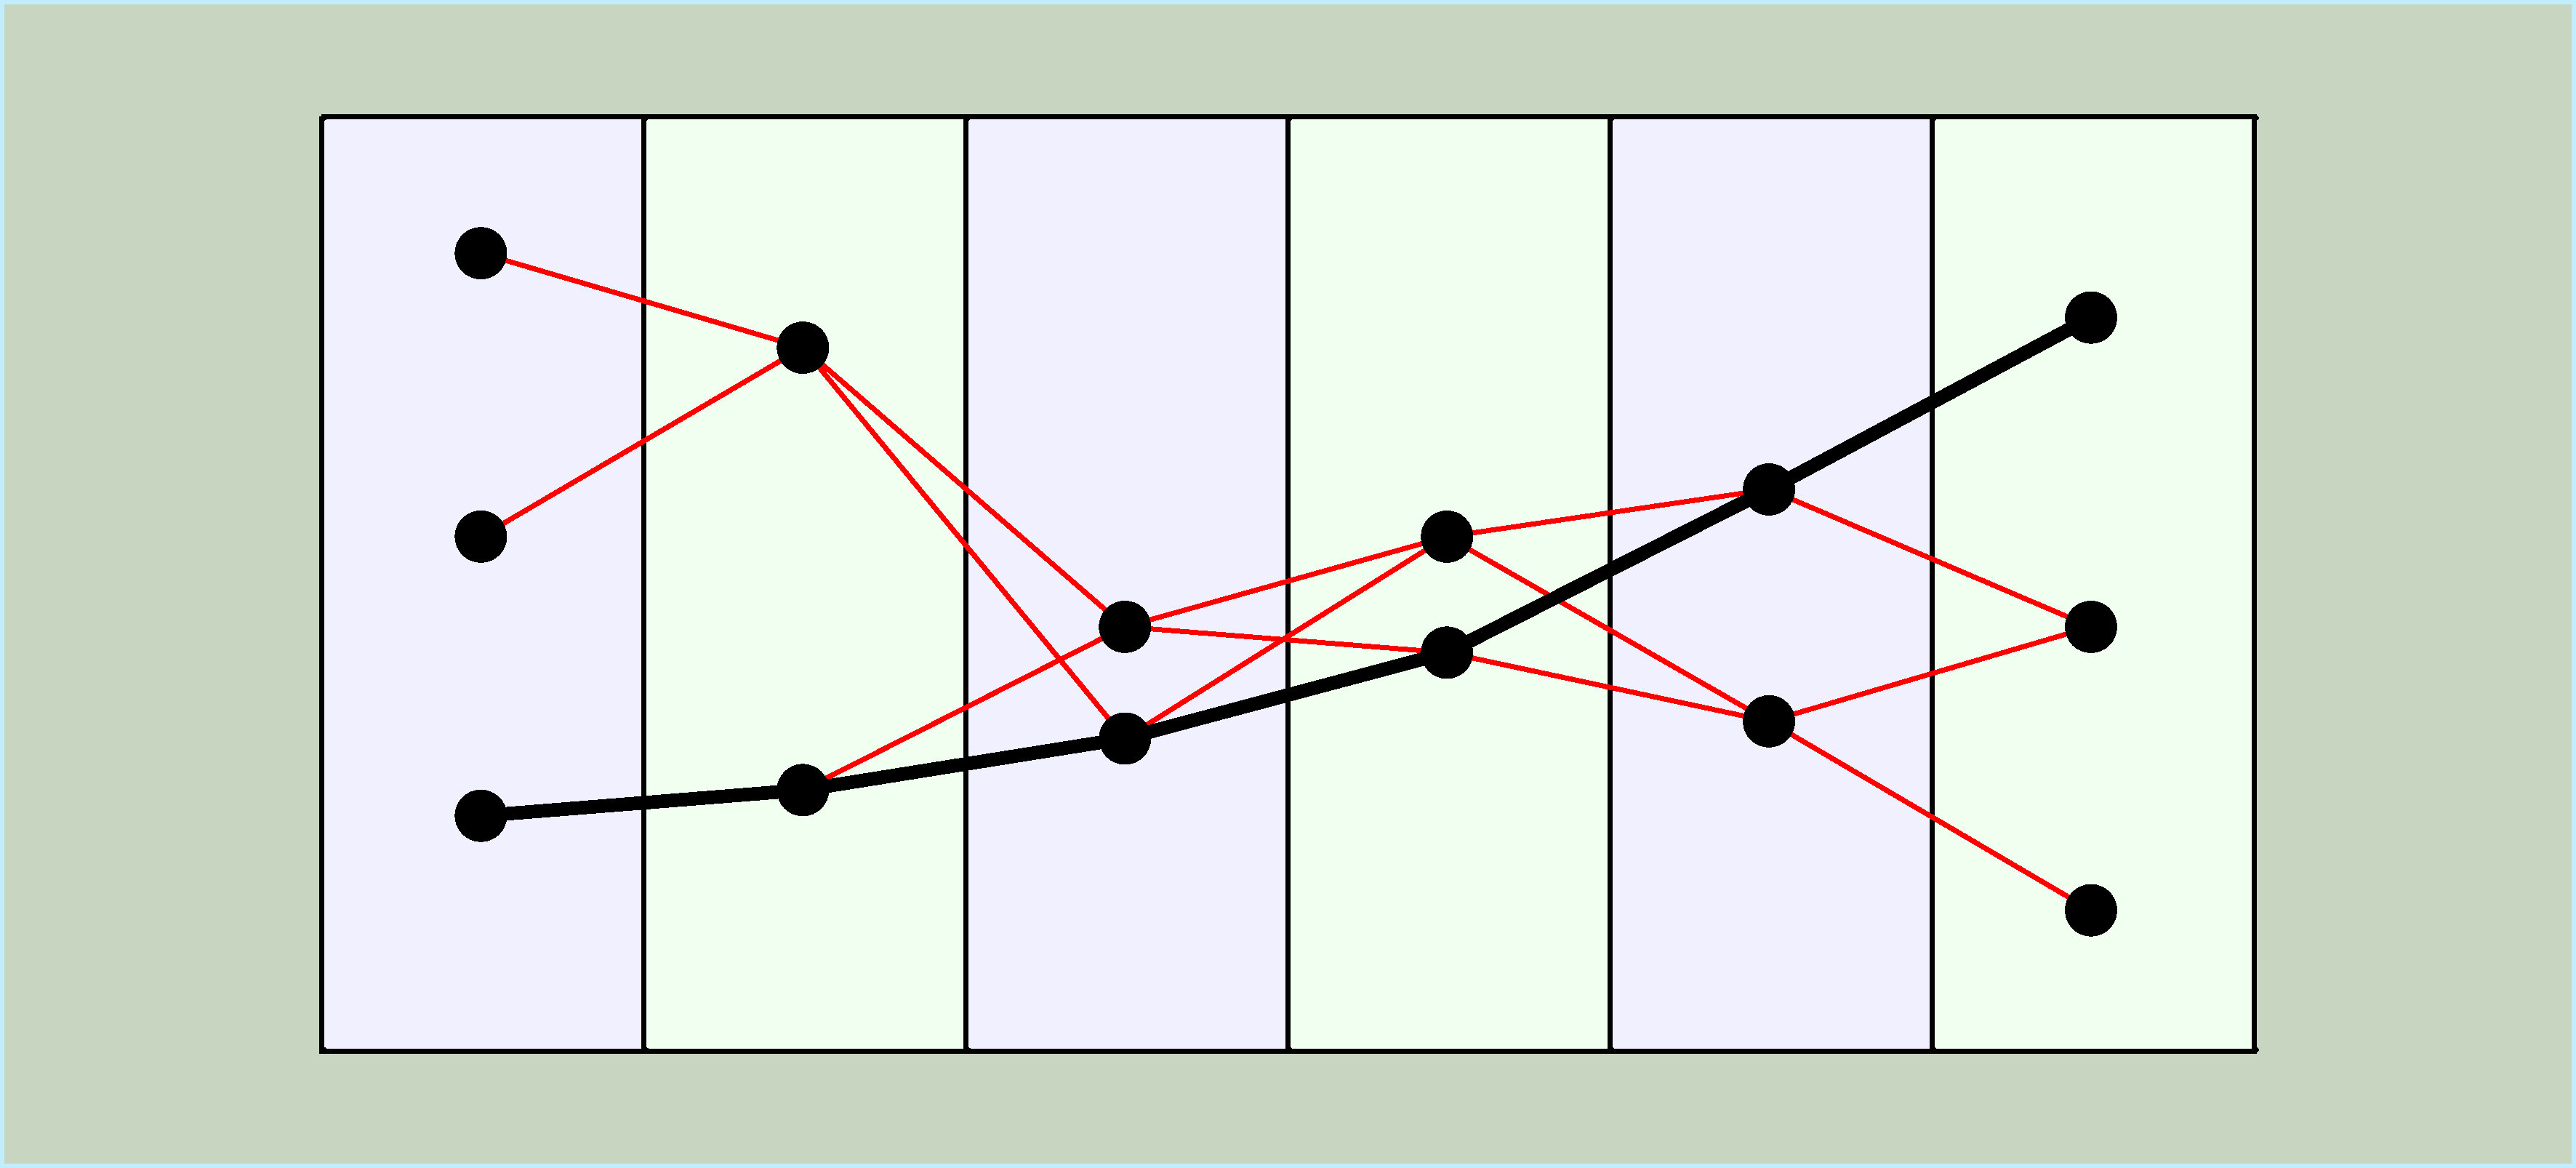
\includegraphics[angle=90,width=1.2in]{images/iden_6_sl.pdf}
  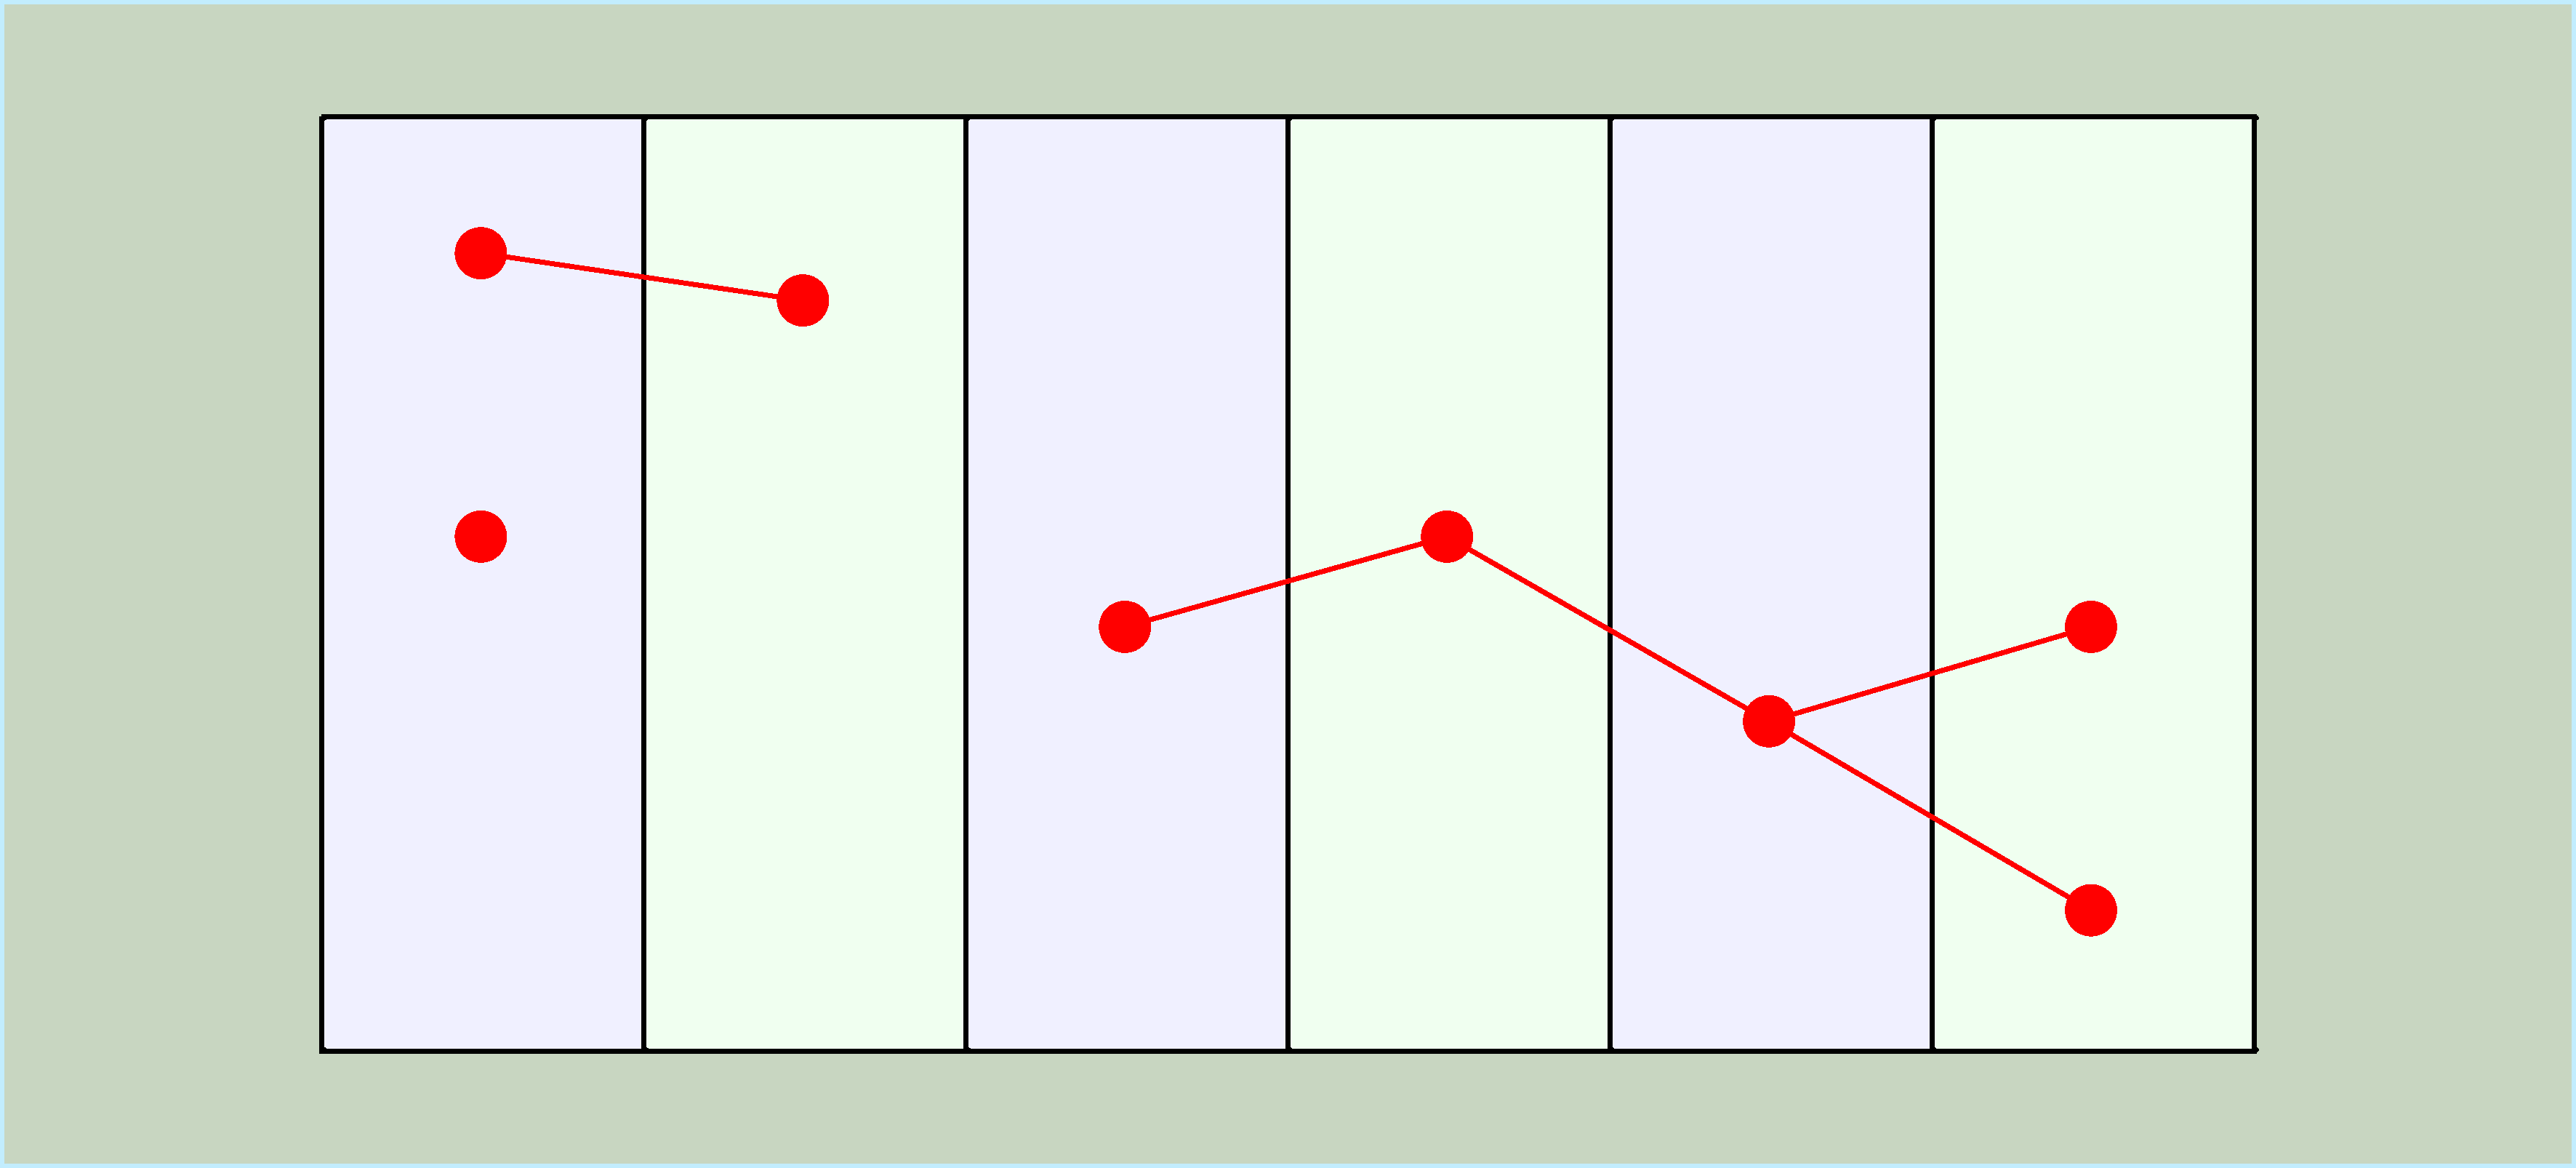
\includegraphics[angle=90,width=1.2in]{images/iden_5_sl_a.pdf}
    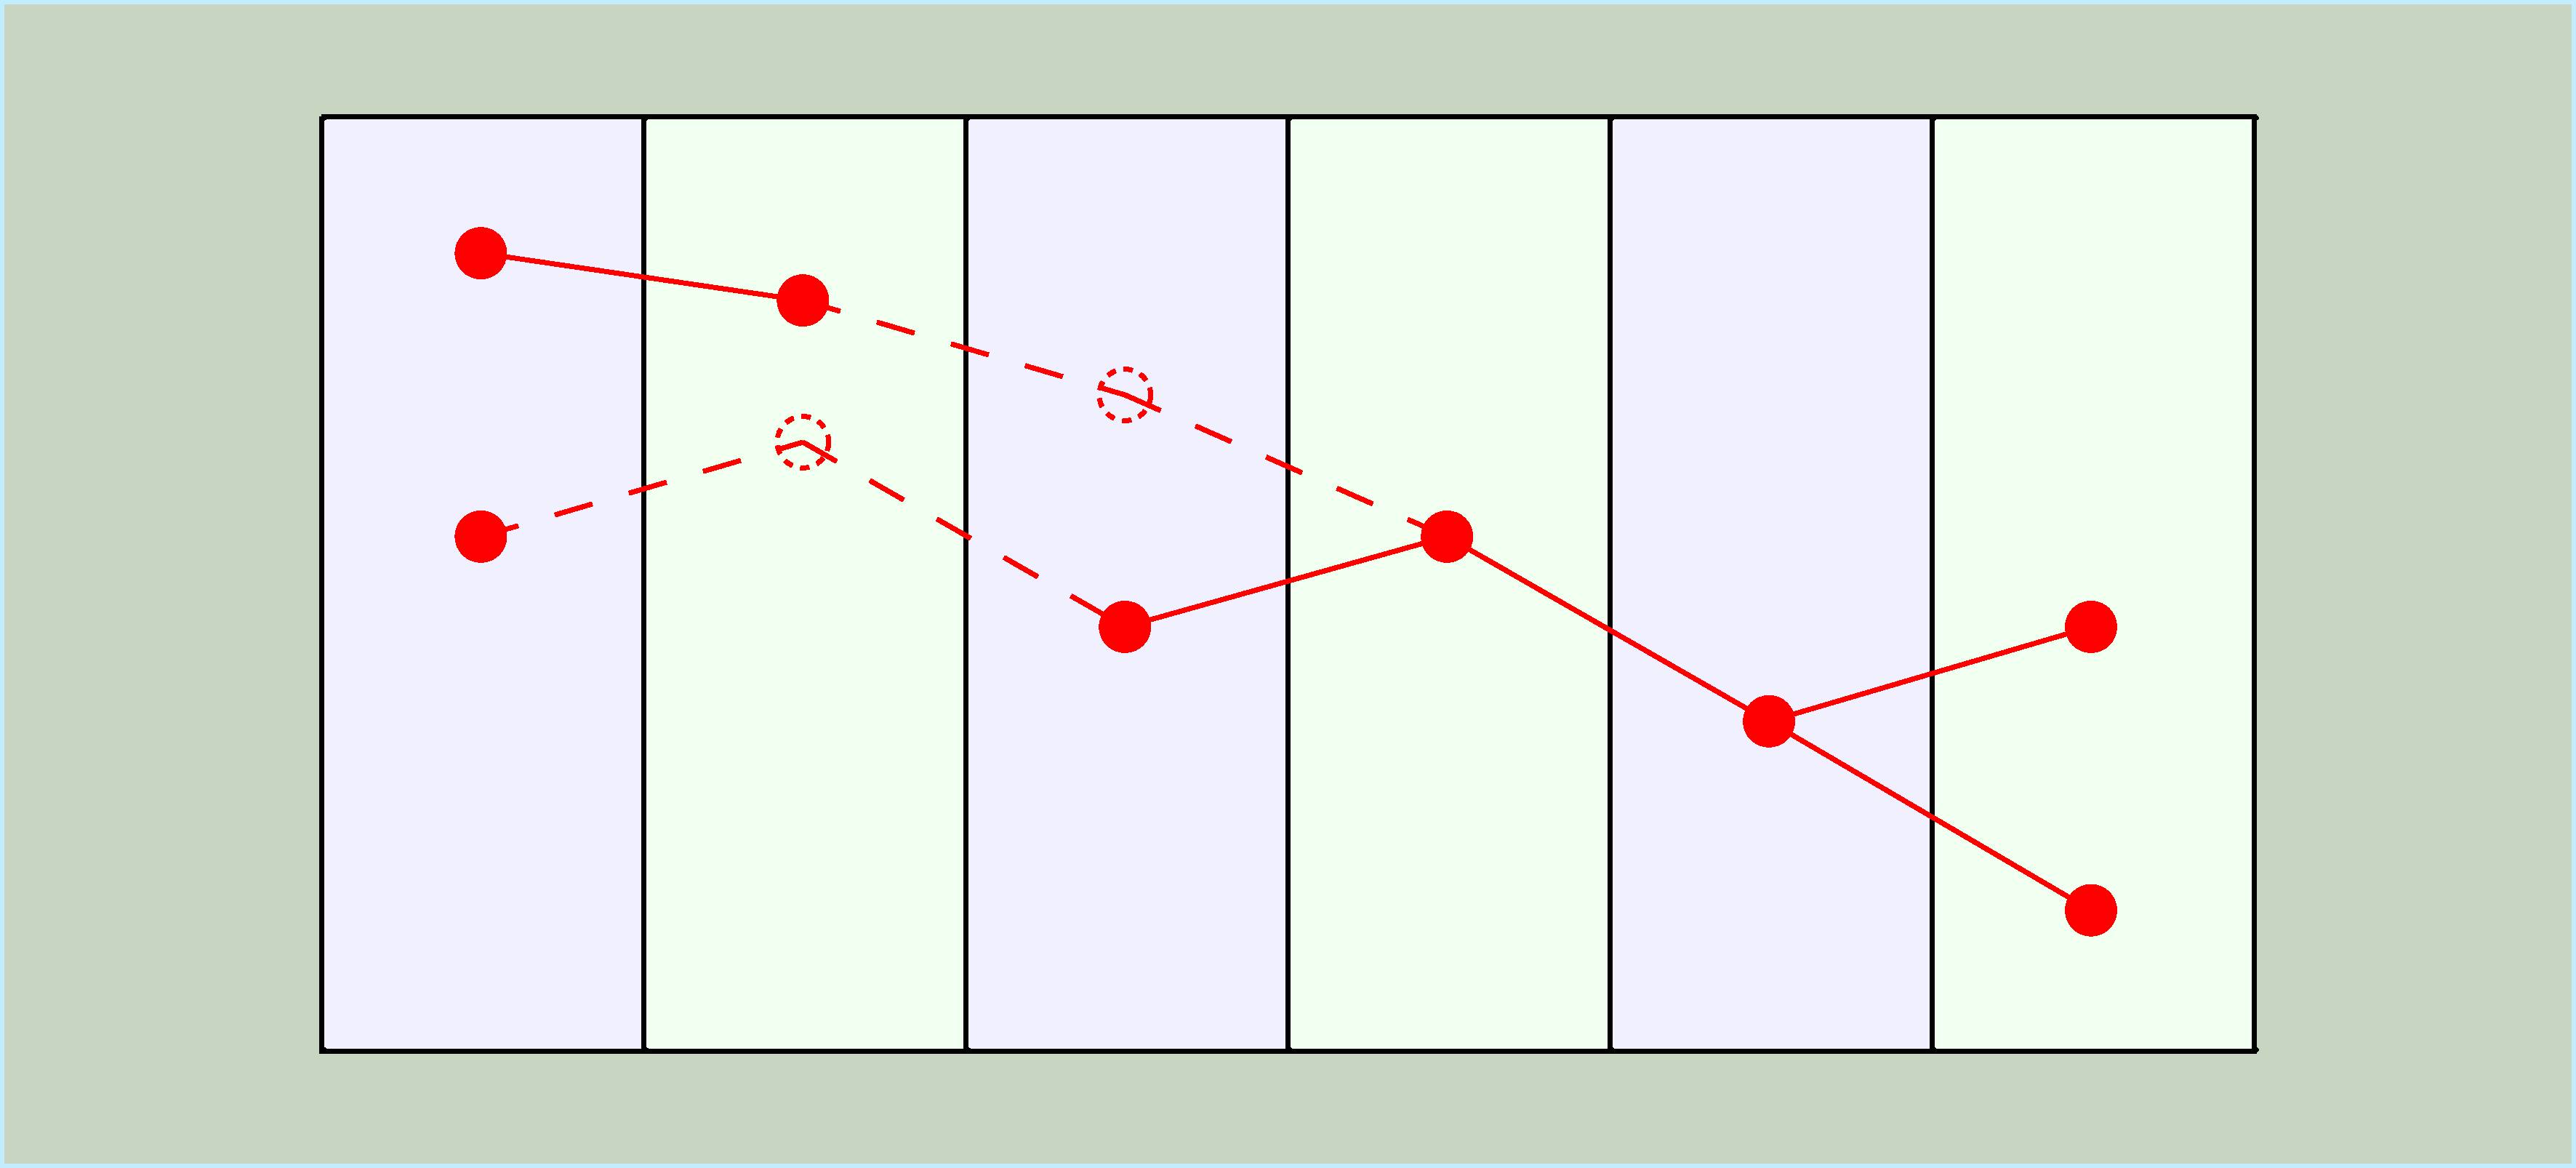
\includegraphics[angle=90,width=1.2in]{images/iden_5_sl_b.pdf}
      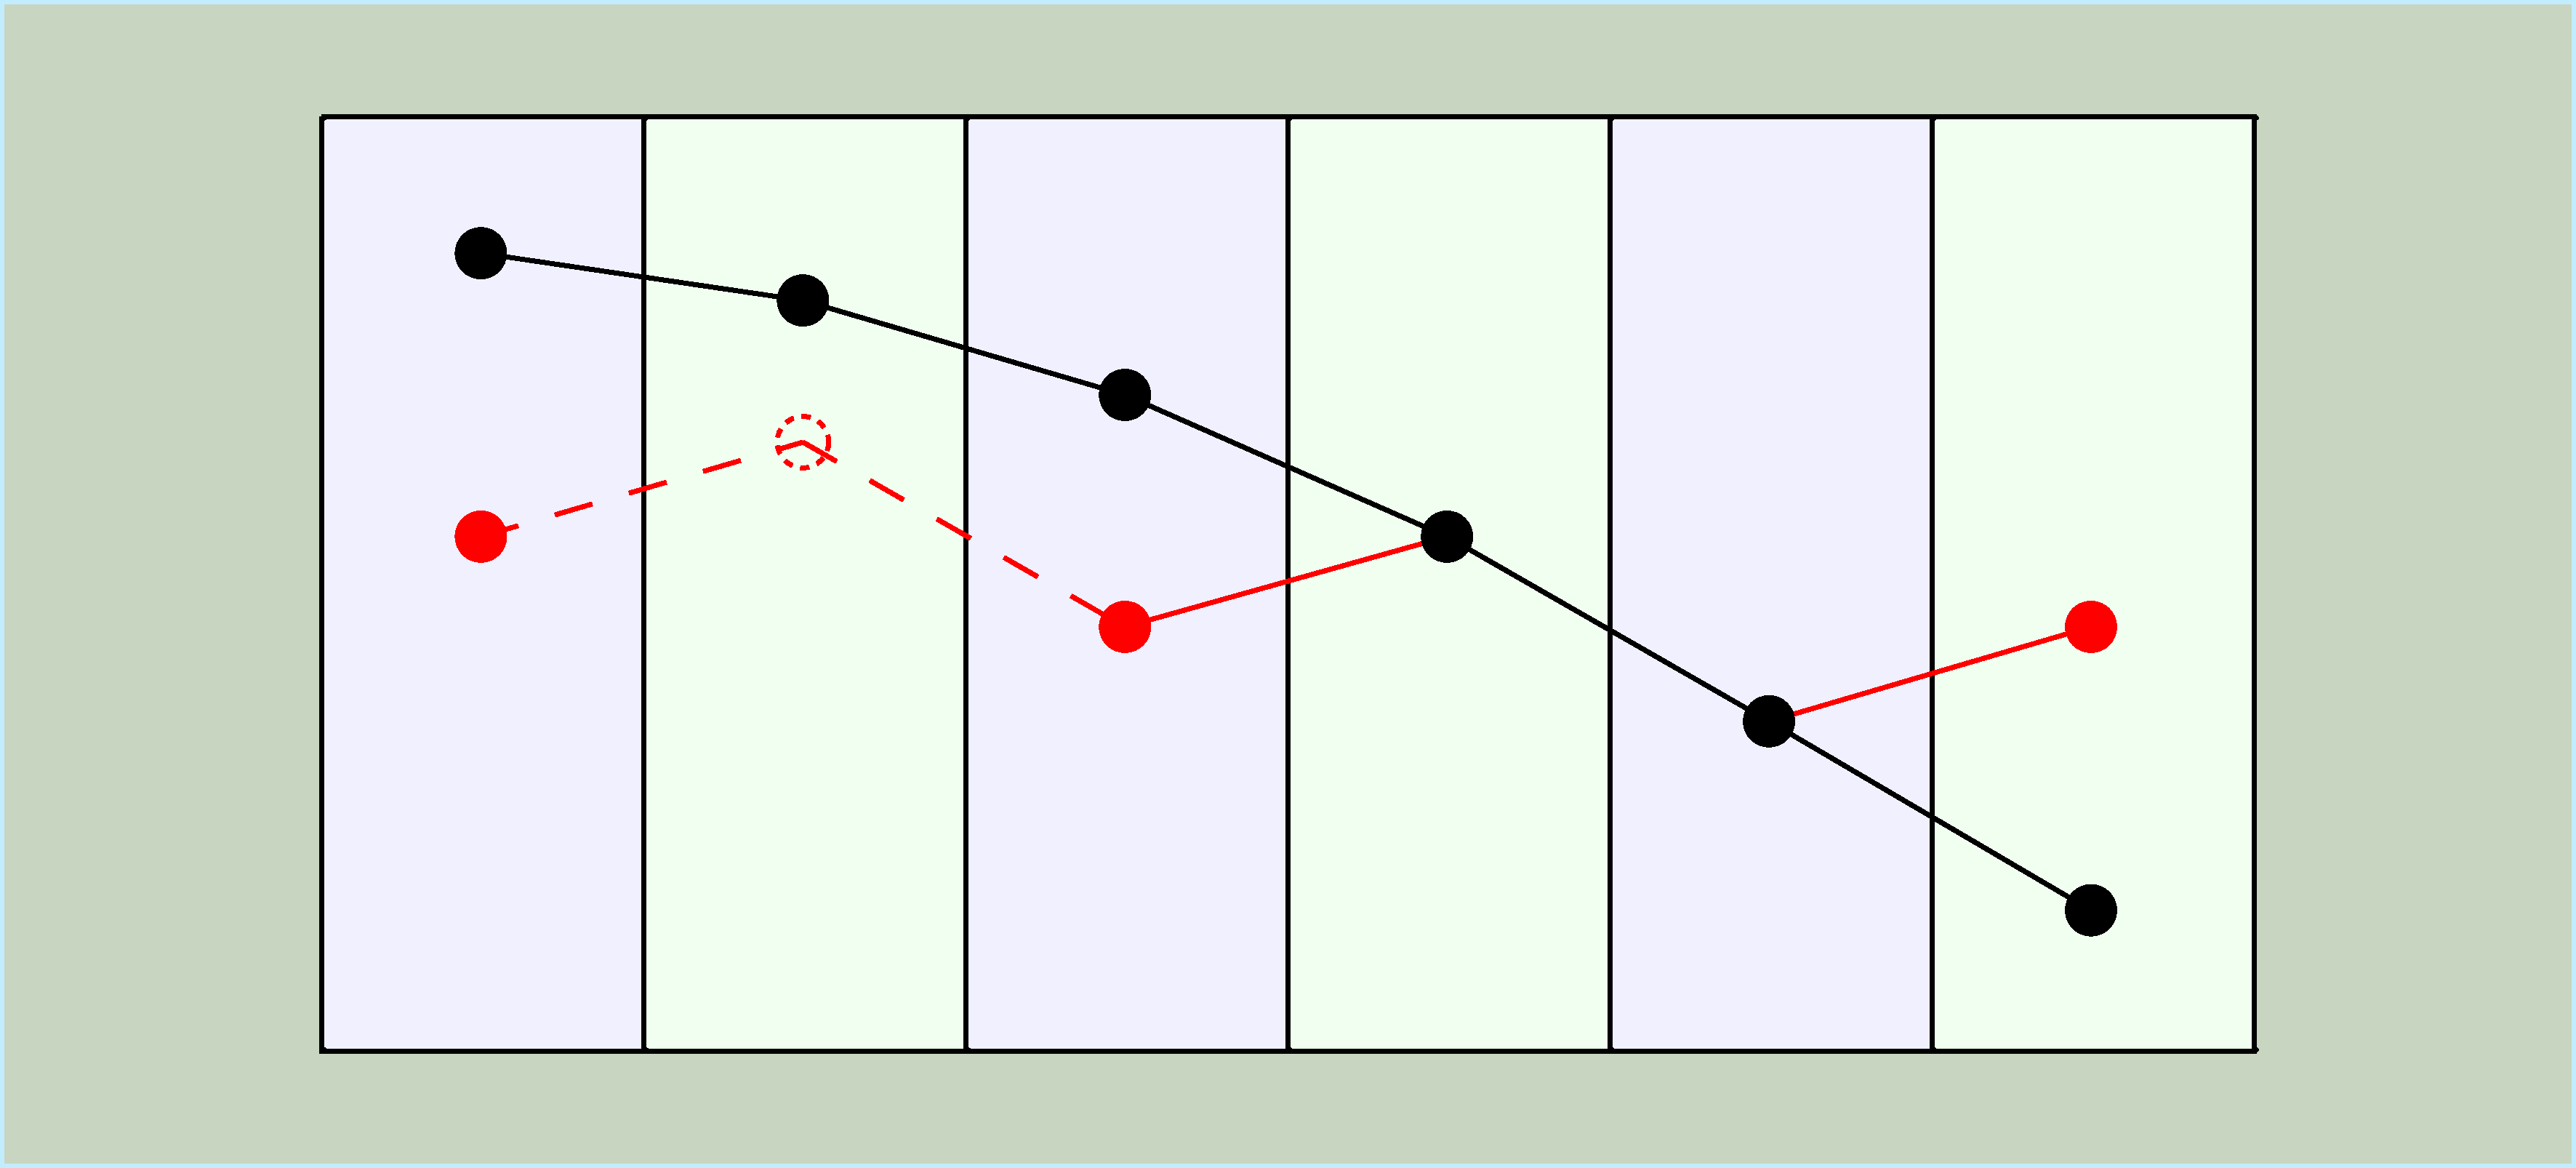
\includegraphics[angle=90,width=1.2in]{images/iden_5_sl_c.pdf}
            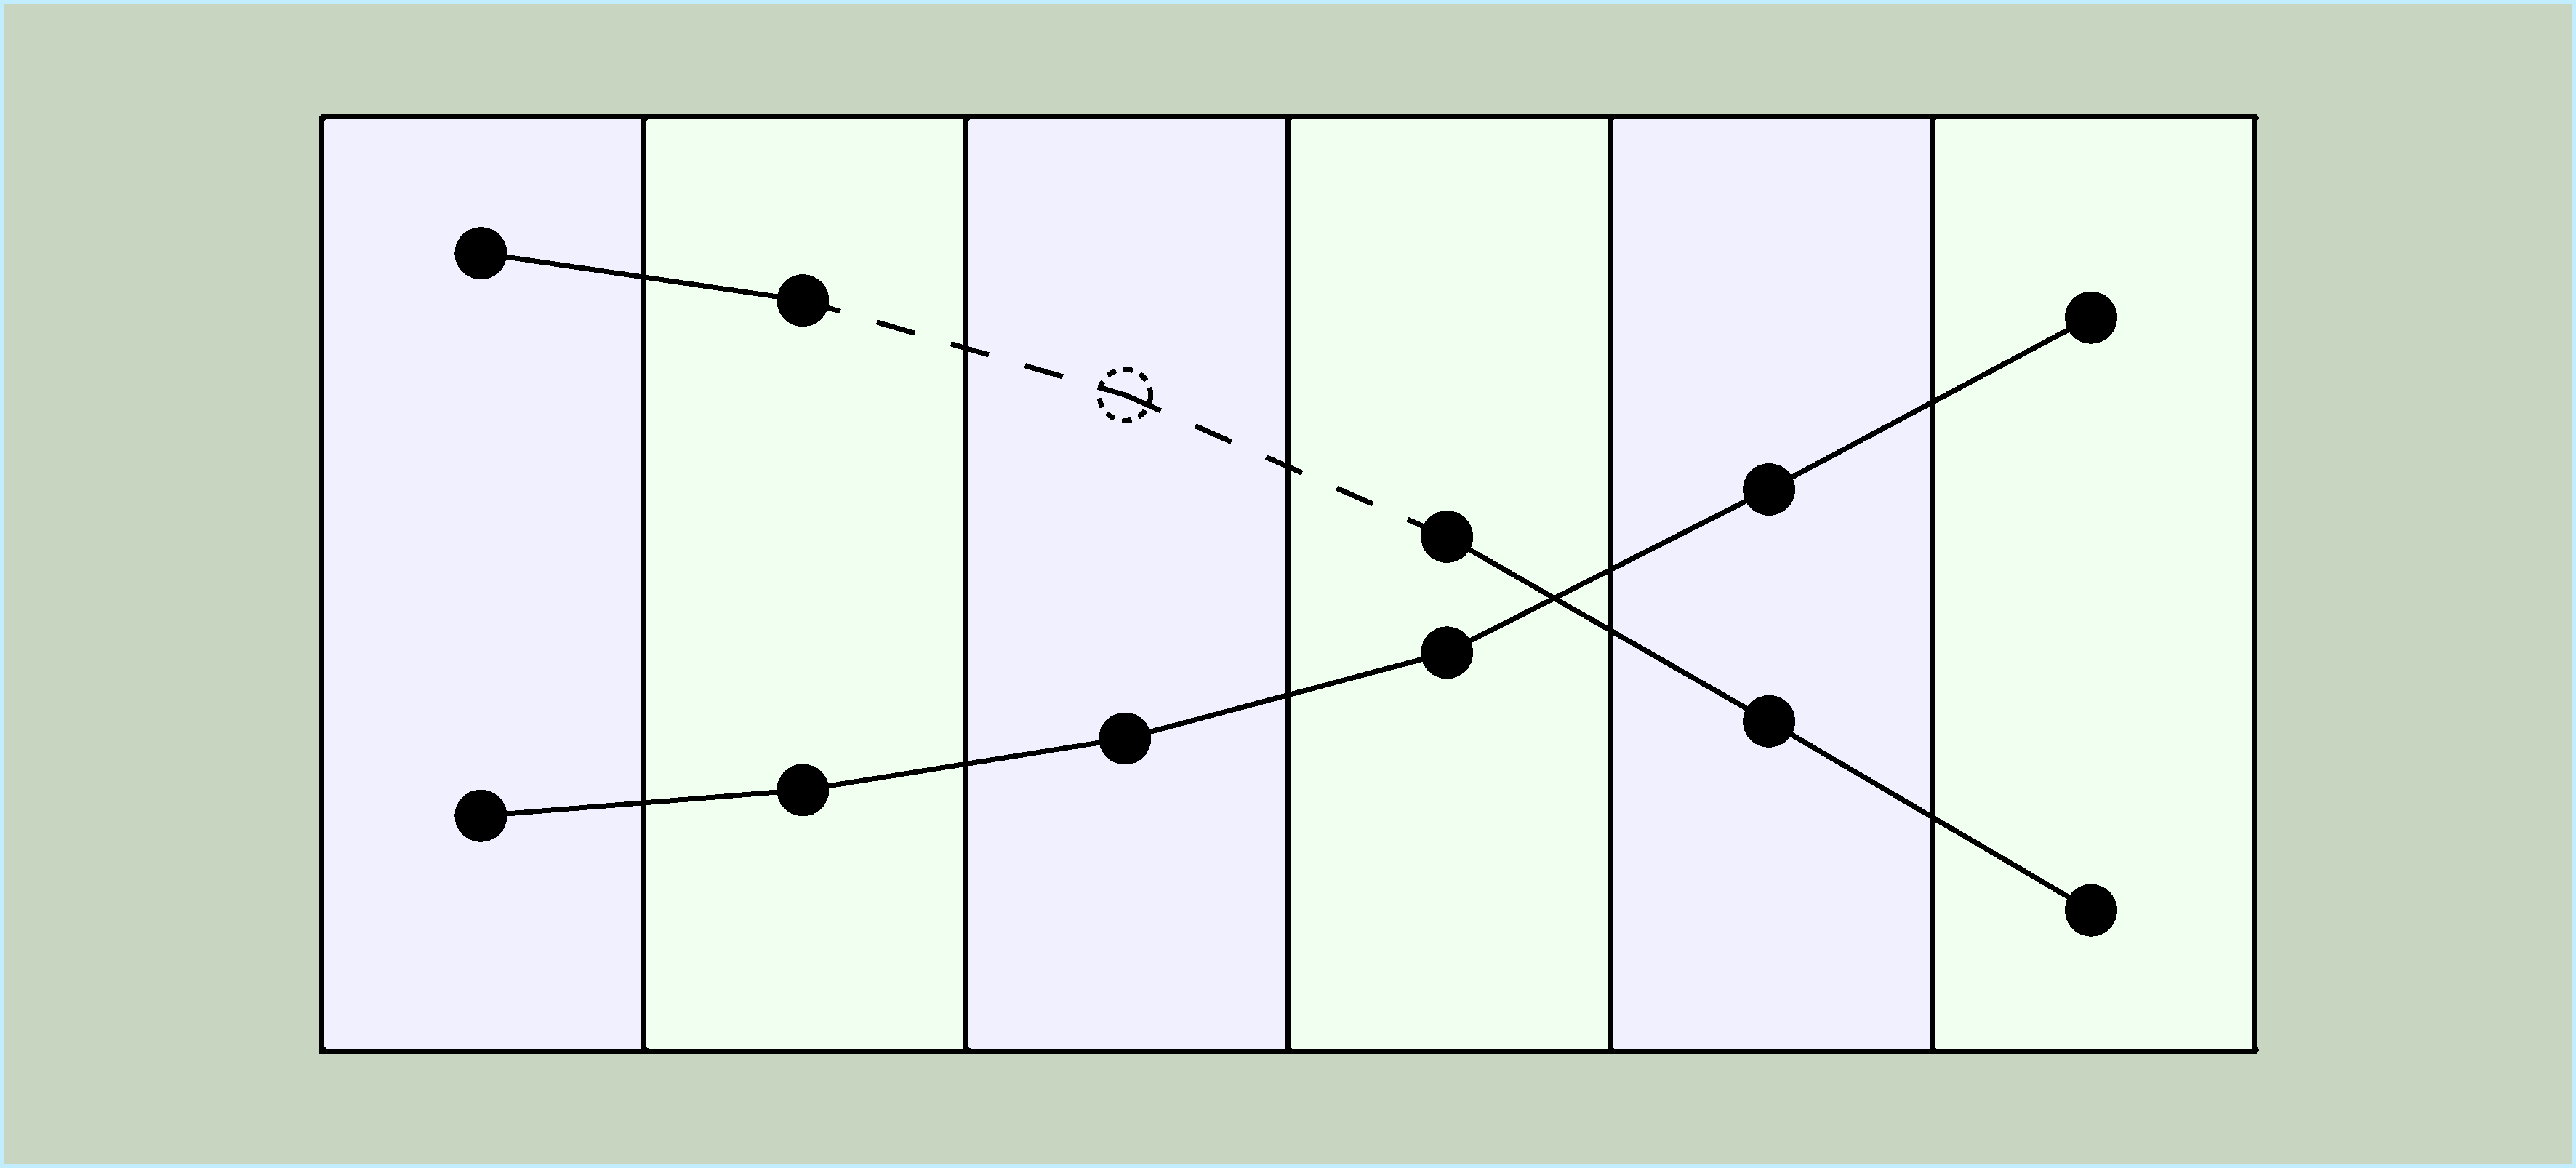
\includegraphics[angle=90,width=1.2in]{images/iden_5_sl_d.pdf}

\caption {Stages of Neural Network track identification procedure. 1) identifying 6 super-layer tracks. 2) removing all hits 
belonging to a identified track and constructing 5 super-layer track candidates. 3) generating pseudo-clusters for 5 super-layer
track candidates using corruption fixing auto-encoder. 4) identify good track candidates from the list of 6 super-layer 
(one of the super-layers is pseudo-cluster) track candidates. 5) isolate both identifies (6 super-layer and 5 super-layer) tracks 
for further fitting with Kalman-Filter.}
 \label{network:procedure}
 \end{center}
\end{figure}

The second stage of track identification starts by constructing a list of track candidates with combinations of 5 clusters 
out of 6 from all existing clusters (one per super-layer). The candidates that share a cluster with tracks
identified at the first stage of classification are removed from the list. For each track candidate with a missing cluster
in one of the super-layers, a pseudo-cluster is generated using the Corruption Auto-Encoder Network and the missing super-layer 
cluster is assigned the inferred value, hence turning all track candidates to 6 cluster track candidates. The 
cured (or fixed) track candidate list is finally passed to the track classifier module described above, which evaluates the list 
isolating candidates with the highest probability of being a good track. 

\subsection{Implementation in reconstruction software}

The CLAS12 reconstruction software framework is a Service Oriented Architecture platform (CLARA \cite{Gyurjyan:2011zz}).
The reconstruction software consists of several microservices, each responsible for processing data from one
detector \cite{Ziegler:2020gsr}. The reconstruction procedure for some of the detector components can also 
be broken down into smaller logical microservices to add some flexibility in changing the implementation of the small parts, 
and provide alternative reconstruction procedures for some of the components.
Reconstruction of tracks in drift chambers is a complex task and consists of several parts.

The first stage of the process, called clustering service, is to isolate clusters
from the hits in drift chambers. Once the clusters are isolated, track candidates are formed from all combinations 
of 6 segments. Once 6 segment tracks have been identified, the remaining segments are then used to form 5 segments combinations. These two steps are known as track-finding or seeding.
Both 6 and 5 segments candidates are fitted defining the hit positions from the wire coordinates (hit based tracking), resulting in a first list of reconstructed tracks.
%The track candidates are analyzed to determine which good candidates from remaining segment 
%combinations of 5 segment tracks are constructed which are also fitted to determine which ones are potential good tracks.
%The later module (hit based tracking) determines good track candidates based only on hit positions of the track candidates (no timing
%informations is used at this level). 

In a second stage of the tracking code (time-based tracking), 
the tracks identified at the previous stage are refitted with a Kalman Filter algorithm, which uses drift time information to refine the hit positions.
This produces the final track list.
%chosen good track candidates are further refined with the Kalman filter by using timing information from each of the sensors (drift chamber wires). By the time the reconstruction code reaches the time based tracking stage, the track candidates have already been defined. 

\begin{figure}[!ht]
\begin{center}
 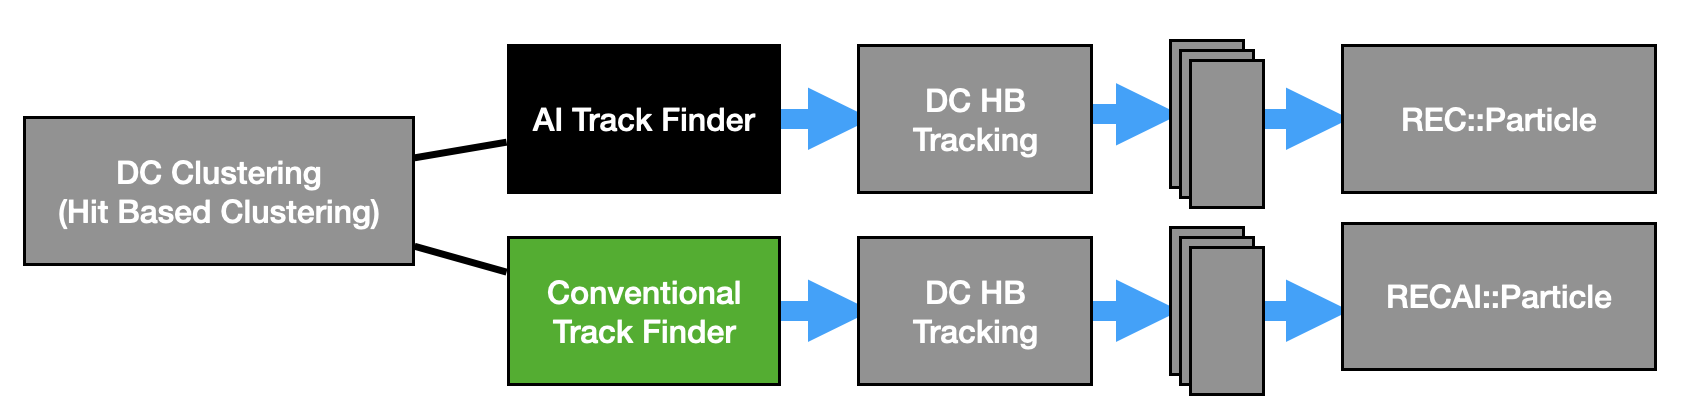
\includegraphics[width=6.0in]{images/recon_diagram.png}
\caption {Diagram of the tracking workflow with Artificial Intelligence included. The Workflow is split into two parallel branches, one where track-finding is done by the conventional algorithm, and one where only AI-isolated tracks are fed to the following stages.}
 \label{recon:diagram}
 \end{center}
\end{figure}

In order to implement our neural network into the reconstruction workflow, we designed two parallel branches in the reconstruction code where we run 
two algorithms to identify good tracks from the candidate lists, one based on the conventional algorithm and one based on the neural network.
The two algorithms store their track suggestions in separate data structures, and pass them to the next stage where track parameters are reconstructed by 
conventional tracking algorithm, first by hit-based fitting and then using the Kalman filter. This approach lets us have two parallel outputs from the tracking code that enables a detailed comparison of the performance of each method.

\subsection{Software Packages}

As mentioned above, CLAS12 reconstruction is implemented in Java. The final implementation of the the track classifier was therefore in Java for easy integration into the reconstruction workflow. The initial tests and prototyping were done using the Keras/TensorFlow (python) package. The final implementation was based on the DeepNetts \cite{Sevarac.Z} community edition library (in native Java) used for both the track candidate classifier and corruption-recovery auto-encoder. DeepNetts is a light weight library with minimal dependencies, which makes it ideal for providing portable code that can be used on variety of platforms without the need of installing large number of platform-dependent packages (like in the case of keras/tensorflow).
The inference procedure was implemented using Efficient Java Matrix Library (EJML) \cite{ejml:2021}, which is optimized for speed and is thread safe, matching the requirements of the CLAS12 reconstruction software.


\section{Analysis of Track Reconstruction with AI}

After implementing the track identification service in the CLAS12 reconstruction software, the outputs
from the conventional tracking algorithm and AI-assisted tracking algorithm were analyzed
event by event to ascertain improvements of tracking. 
 
 \subsection{Particle Reconstruction efficiency}
 
 The Neural Network for track classification was trained on experimental data after it was processed with conventional tracking 
 reconstruction. Tracks that have ``good'' fit quality and were tracked back to the target were used as training samples for both 
 the MLP classifier and Auto-Encoder corruption-recovery network. For more detailed analysis of tracking reconstruction performance with and without assistance from artificial intelligence we processed one run at nominal luminosity (45 nA) to compare performances.
 
 %The efficiency of track reconstruction was obtained for separate track topologies (6 super-layer and 5 super-layer).
 \begin{figure}[!ht]
\begin{center}
% 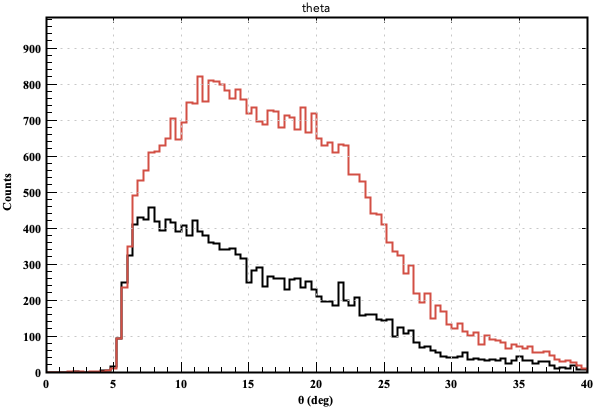
\includegraphics[width=2.0in]{images/pos_theta_5SL.png}
  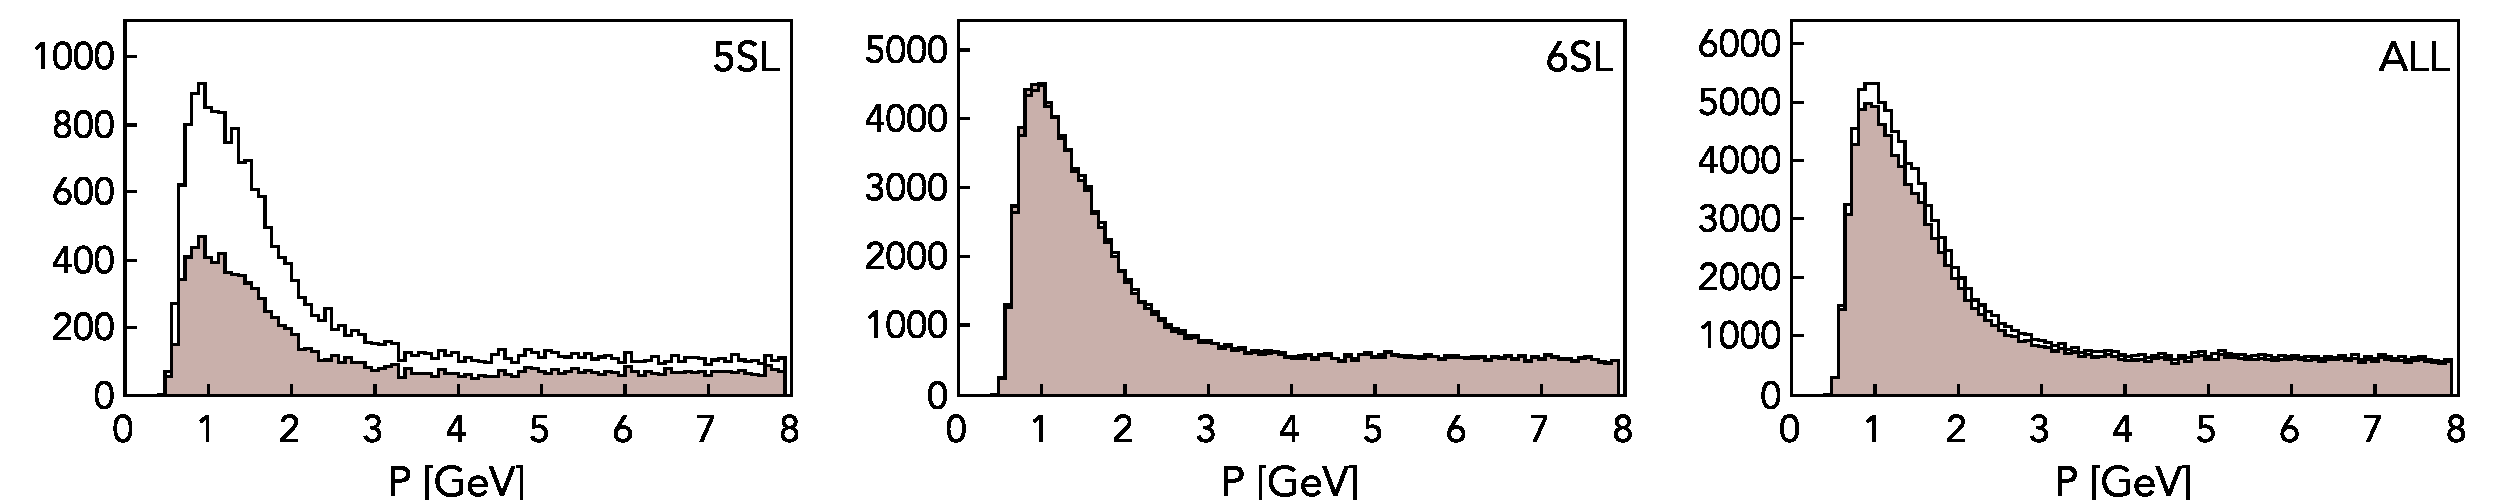
\includegraphics[width=6.5in]{images/figure_p.pdf}
  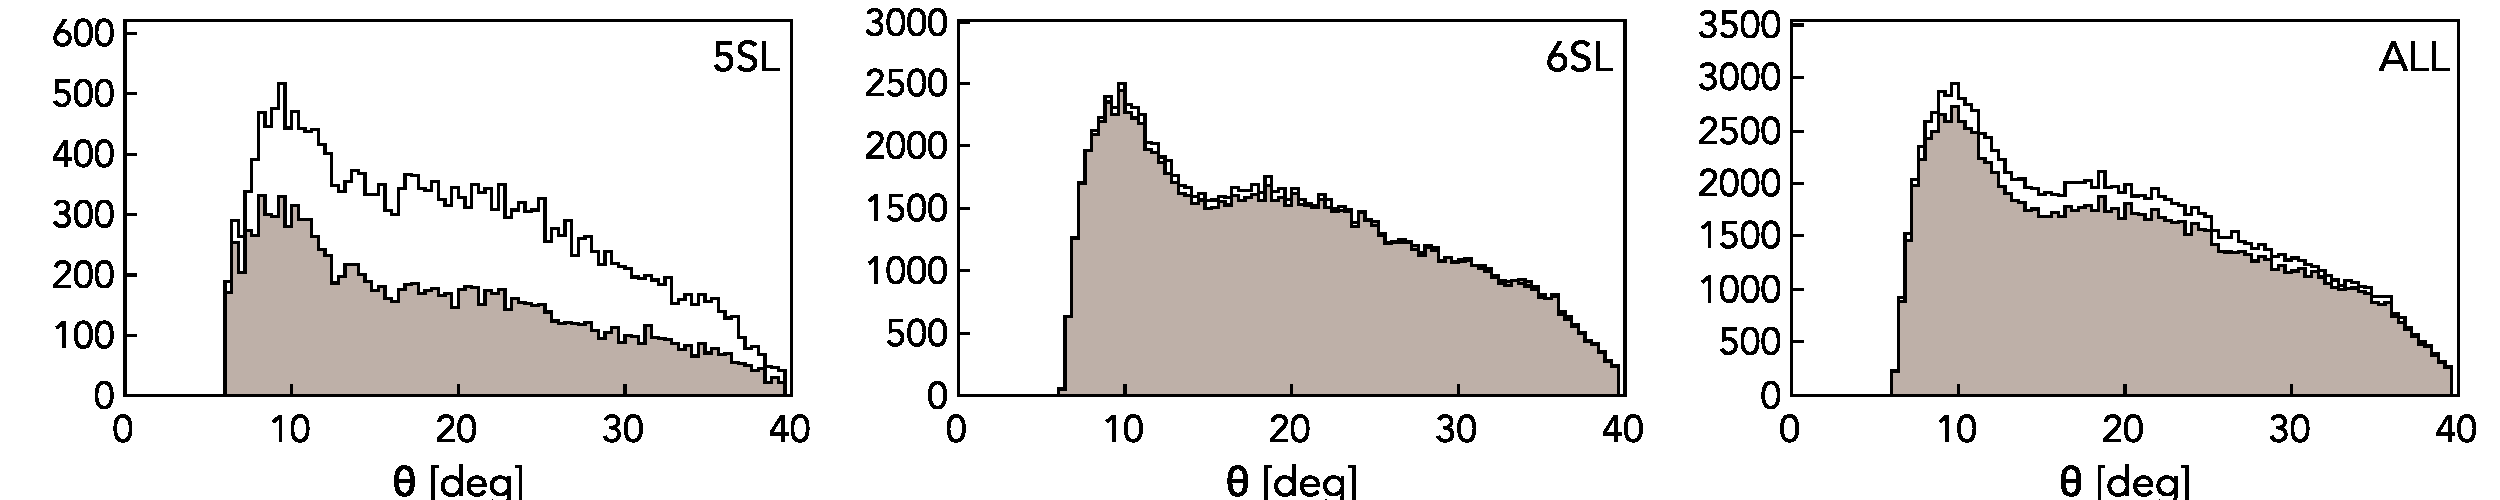
\includegraphics[width=6.5in]{images/figure_theta.pdf}
    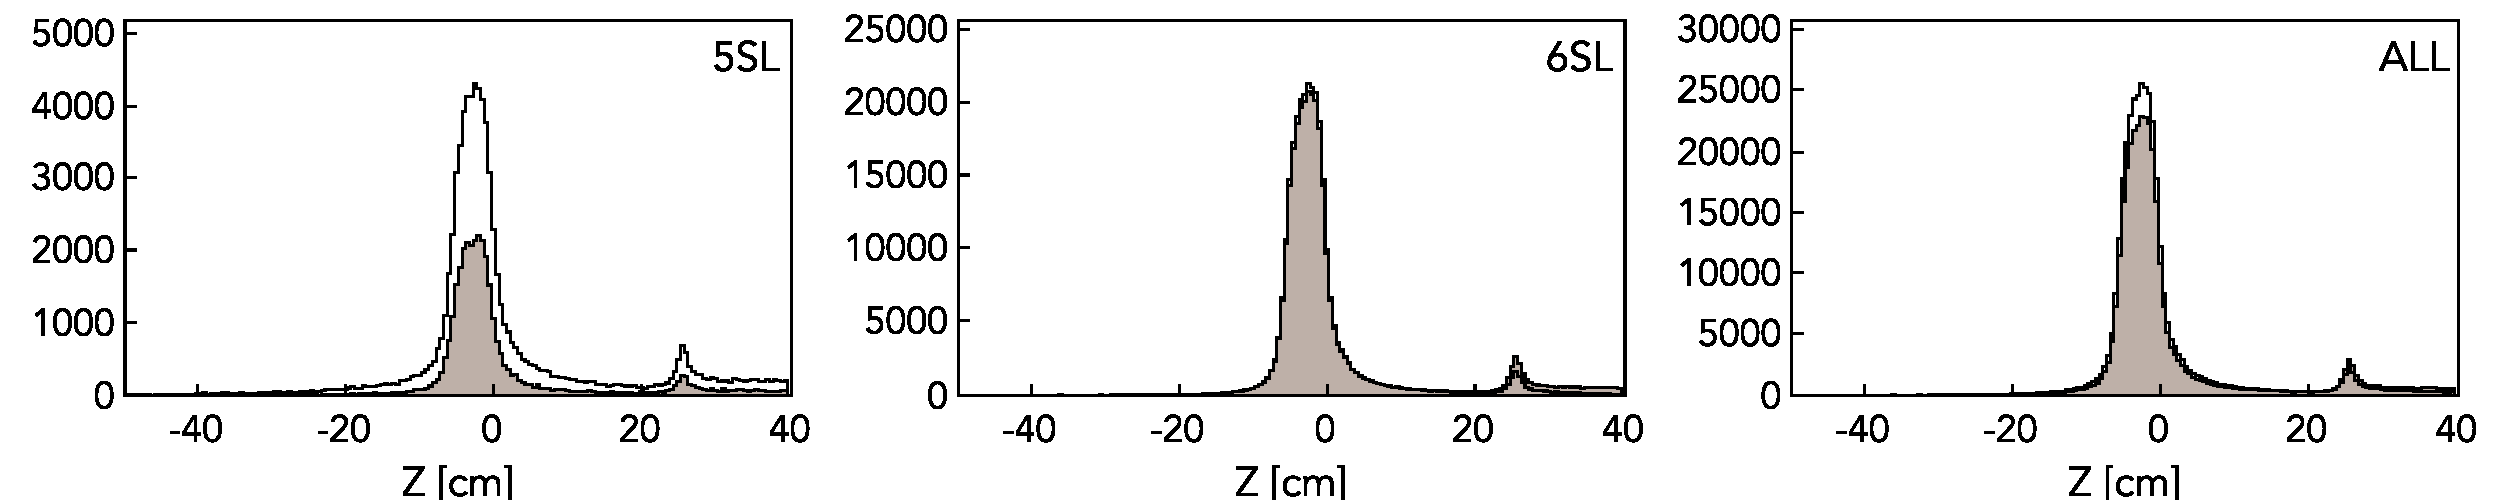
\includegraphics[width=6.5in]{images/figure_vz.pdf}
\caption { Comparison of number of tracks reconstructed with the conventional algorithm (filled histograms) vs AI-assisted tracking code (open black outline histograms) as a function of momentum, polar angle and particle interaction vertex. The comparison is shown for 5 super-layer, 6 super-layer tracks (left two columns), and the total number (right column).}
 \label{track:efficiency}
 \end{center}
\end{figure}

The results are shown on Figure~\ref{track:efficiency}, where dependence of number of reconstructed negatively charged 
 tracks are shown as a function of particle momentum (top row), polar angle in laboratory frame (bottom row) and interaction
 vertex (middle row). The reconstructed distributions from conventional tracking are plotted with filled histograms and the
 tracks reconstructed using assistance from AI are plotted with solid lines. As can be seen from the figure, there is a large gain 
 in the number of reconstructed tracks with the 5 super-layer configuration compared to full 6 super-layer tracks. Typically for nominal 
 45 nA experimental data increase in track efficiency for 6 super-layers tracks averages about $3\%-6\%$, while for 5 super-layer
 tracks the increase is in the order of $70\%-120\%$. In normal data reconstruction, tracks that are identified with 5 super-layers
 usually comprise about $10\%$ of all reconstructed tracks, and a significant increase in identification of such tracks leads to 
 overall tracking efficiency increase of $12\%-15\%$. 
 
 \begin{table}[!h]
 \begin{center}
 \begin{tabular}{|l|c|c|c|c|}
 \hline
 Track Configuration & Conventional & AI Assisted & Gain & Relative \\
 \hline
 \hline
 6 Super-Layer & 242,145 & 256,175 & 14030 & 1.0579 \\
 5 Super-Layer & 24,155 & 52,839 & 28684 & 2.1875 \\
 All & 267,339 & 309,058 & 51719 & 1.1561 \\
 \hline
 \end{tabular}
 \end{center}
 \caption{Summary of reconstructed tracks and gain with assistance from Artificial Intelligence.}
 \label{tbl:summary}
 \end{table}
 
The comparison of 5 and 6-segment track statistics and their relative gain is summarized in Table~\ref{tbl:summary}.
As can be seen from the table the gain in only 6-segment tracks is about $5.7\%$ but with significant gain in 5 super-layer tracks 
the overall gain in reconstructed tracks elevates to $>15\%$. These results are intuitive since track candidates composed of 5
super-layers with the same number of clusters in each super-layer are significantly higher than 6 super-layer track candidates, and 
in our tests AI performs better in choosing the right combination with increasing combinatorics.
 
\subsection{Luminosity Dependence}

Track reconstruction efficiency increased with AI-assisted tracking, since AI can better identify tracks
from a pool of candidates. One would expect that if the number of combinations decrease the efficiency 
of the conventional track selection algorithm should approach the efficiency of AI-assisted track identification.
Similarly, when the number of combinations increases the advantage of AI over the conventional algorithm should
increase. Based on this we expect AI to perform better in higher background settings. To evaluate AI-assisted
tracking efficiency dependence on background we analyzed several different runs that were taken in different 
conditions (i.e. beam current) ranging from $5~nA$ to $70~nA$. To measure tracking efficiency we first calculated
the number of electrons ($N_e$) detected in the data sample analyzed (typically one run) and then the number of positive and negative
 hadrons that were detected with the electron inclusively ($N_{h^+e}$ and $N_{h^-e}$ respectively).

Then the efficiency for the data set was calculated as:

\begin{equation}
L_t^+ = \frac{N_{h^+e}}{N_e} , L_t^- = \frac{N_{h^-e}}{N_e} 
\end{equation}

where $L_t^+$ is the efficiency of positive particles and $L_t^-$ is the efficiency of negatively charged particles respectively. 
In order to estimate the charged particle reconstruction efficiency as a function of the beam current, the multiplicity, $L_t^{+/-}$, is fitted with a linear function:
\begin{equation}
L_t^{+/-} = a + c\times I 
\end{equation}

Here $a$ and $c$ are the fit parameters and $I$ is the beam current. Then it was assumed that the reconstruction efficiency, $E=1$ at $I=0$ nA:

\begin{equation}
E^{+/-} = 1 + b \times I 
\end{equation}

with $b=\frac{c}{a}$. The slope parameter b is the rate of the reconstruction inefficiency as a function of the beam current \cite{Stepanyan:2020bg}.
%The all points were 
%fitted with linear function $L=a+bx$, where $a$ is the intercept 
 
 \begin{figure}[!ht]
\begin{center}
 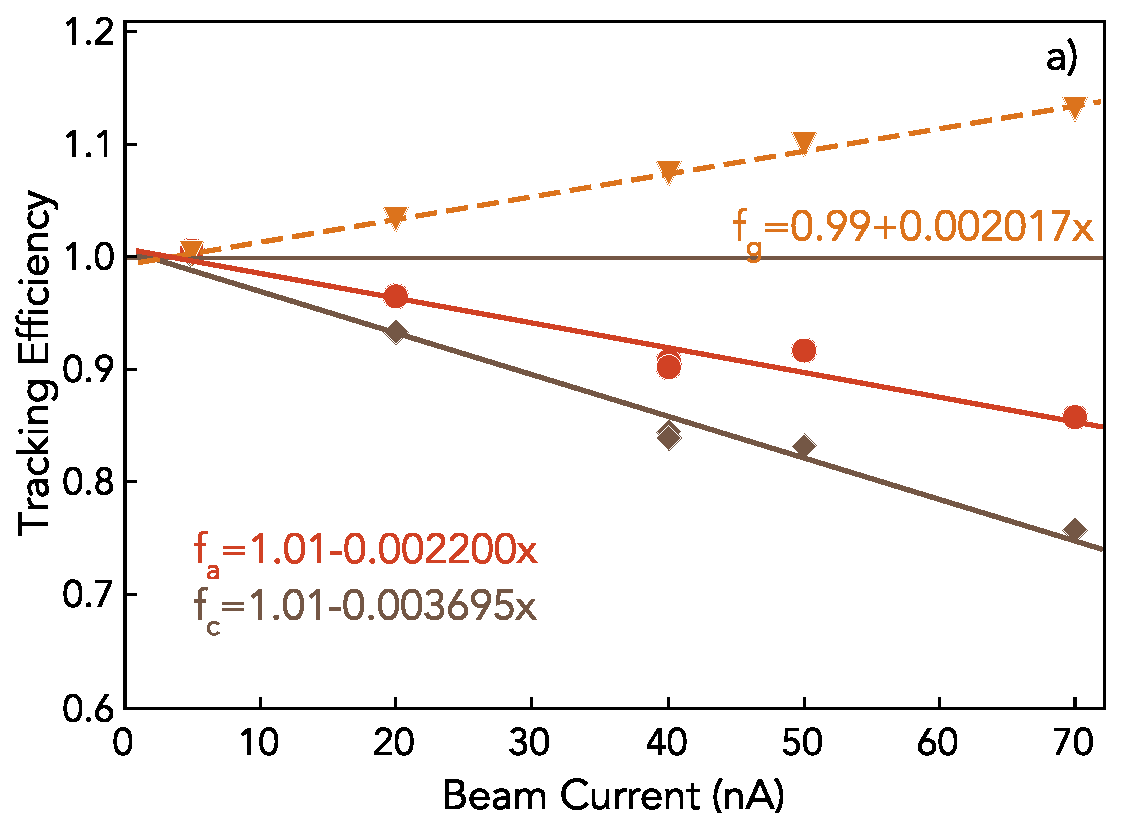
\includegraphics[width=3.0in]{images/figure_lscan_pos.pdf}
 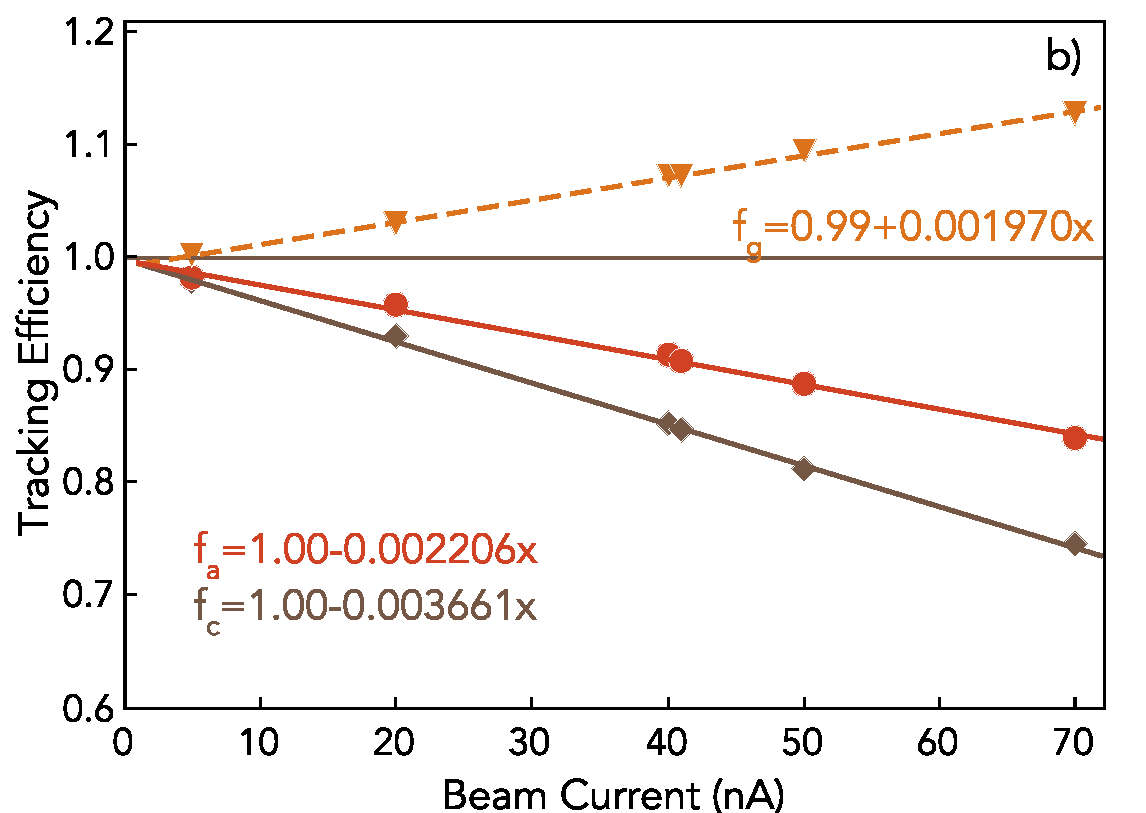
\includegraphics[width=3.0in]{images/figure_lscan_neg.pdf}
\caption {Tracking efficiency for positively and negatively charged particles as a function of beam current (luminosity).  Conventional algorithm 
track reconstruction efficiency (diamonds) is compared to AI-assisted track reconstruction efficiency (circles). }
 \label{lumi:scan}
 \end{center}
\end{figure}

The comparison of tracking efficiency as a function of beam current (luminosity) can be seen on Figure~\ref{lumi:scan} where $E^{+/-}$ are shown for positively and negatively charged particles separately. As can be seen from the figure, AI-assisted tracking performs significantly better for any given luminosity (beam current) and the decrease of efficiency is much slower as a function of luminosity, $0.22\%$ per nA versus $0.40\%$ per nA for conventional tracking. This is expected and consistent with the assumption that with increased combinatorial background (increased number of track candidates to consider), AI performs better in choosing the best track candidate. We established that AI-assisted
tracking leads to more tracks reconstructed for any given beam current setting. The next thing to check is what is the impact of increased track reconstruction efficiency on physics analysis.
% and if there is increase in physics outcome for the CLAS12 experimental setup.

\subsection{Physics Impact}

To measure practical implications of track reconstruction efficiency improvement on physics outcome we analyzed 
two event topologies with two particle and three particles in the final state respectively. The data for analysis were 
taken with $10.5~GeV$ electron beam incident on $20~cm$ liquid hydrogen target, with a beam current of $45~nA$
(typical for CLAS12 experimental running). We selected events where an electron was detected in the forward detector, and 
then isolated events where there was an additional negatively charged pion ($\pi^-$) along with an electron and no other 
charged particle. The second topology required two pions along with electron, one positively charged and one 
negatively charged. The two chosen topologies are denoted by $H(e,e'\pi^-X)$ and $H(e,e'\pi^+\pi^-X)$. In both cases 
there is a visible peak of a missing proton that we can use to measure the impact of efficiency on physics outcome. 

 \begin{figure}[!ht]
\begin{center}
 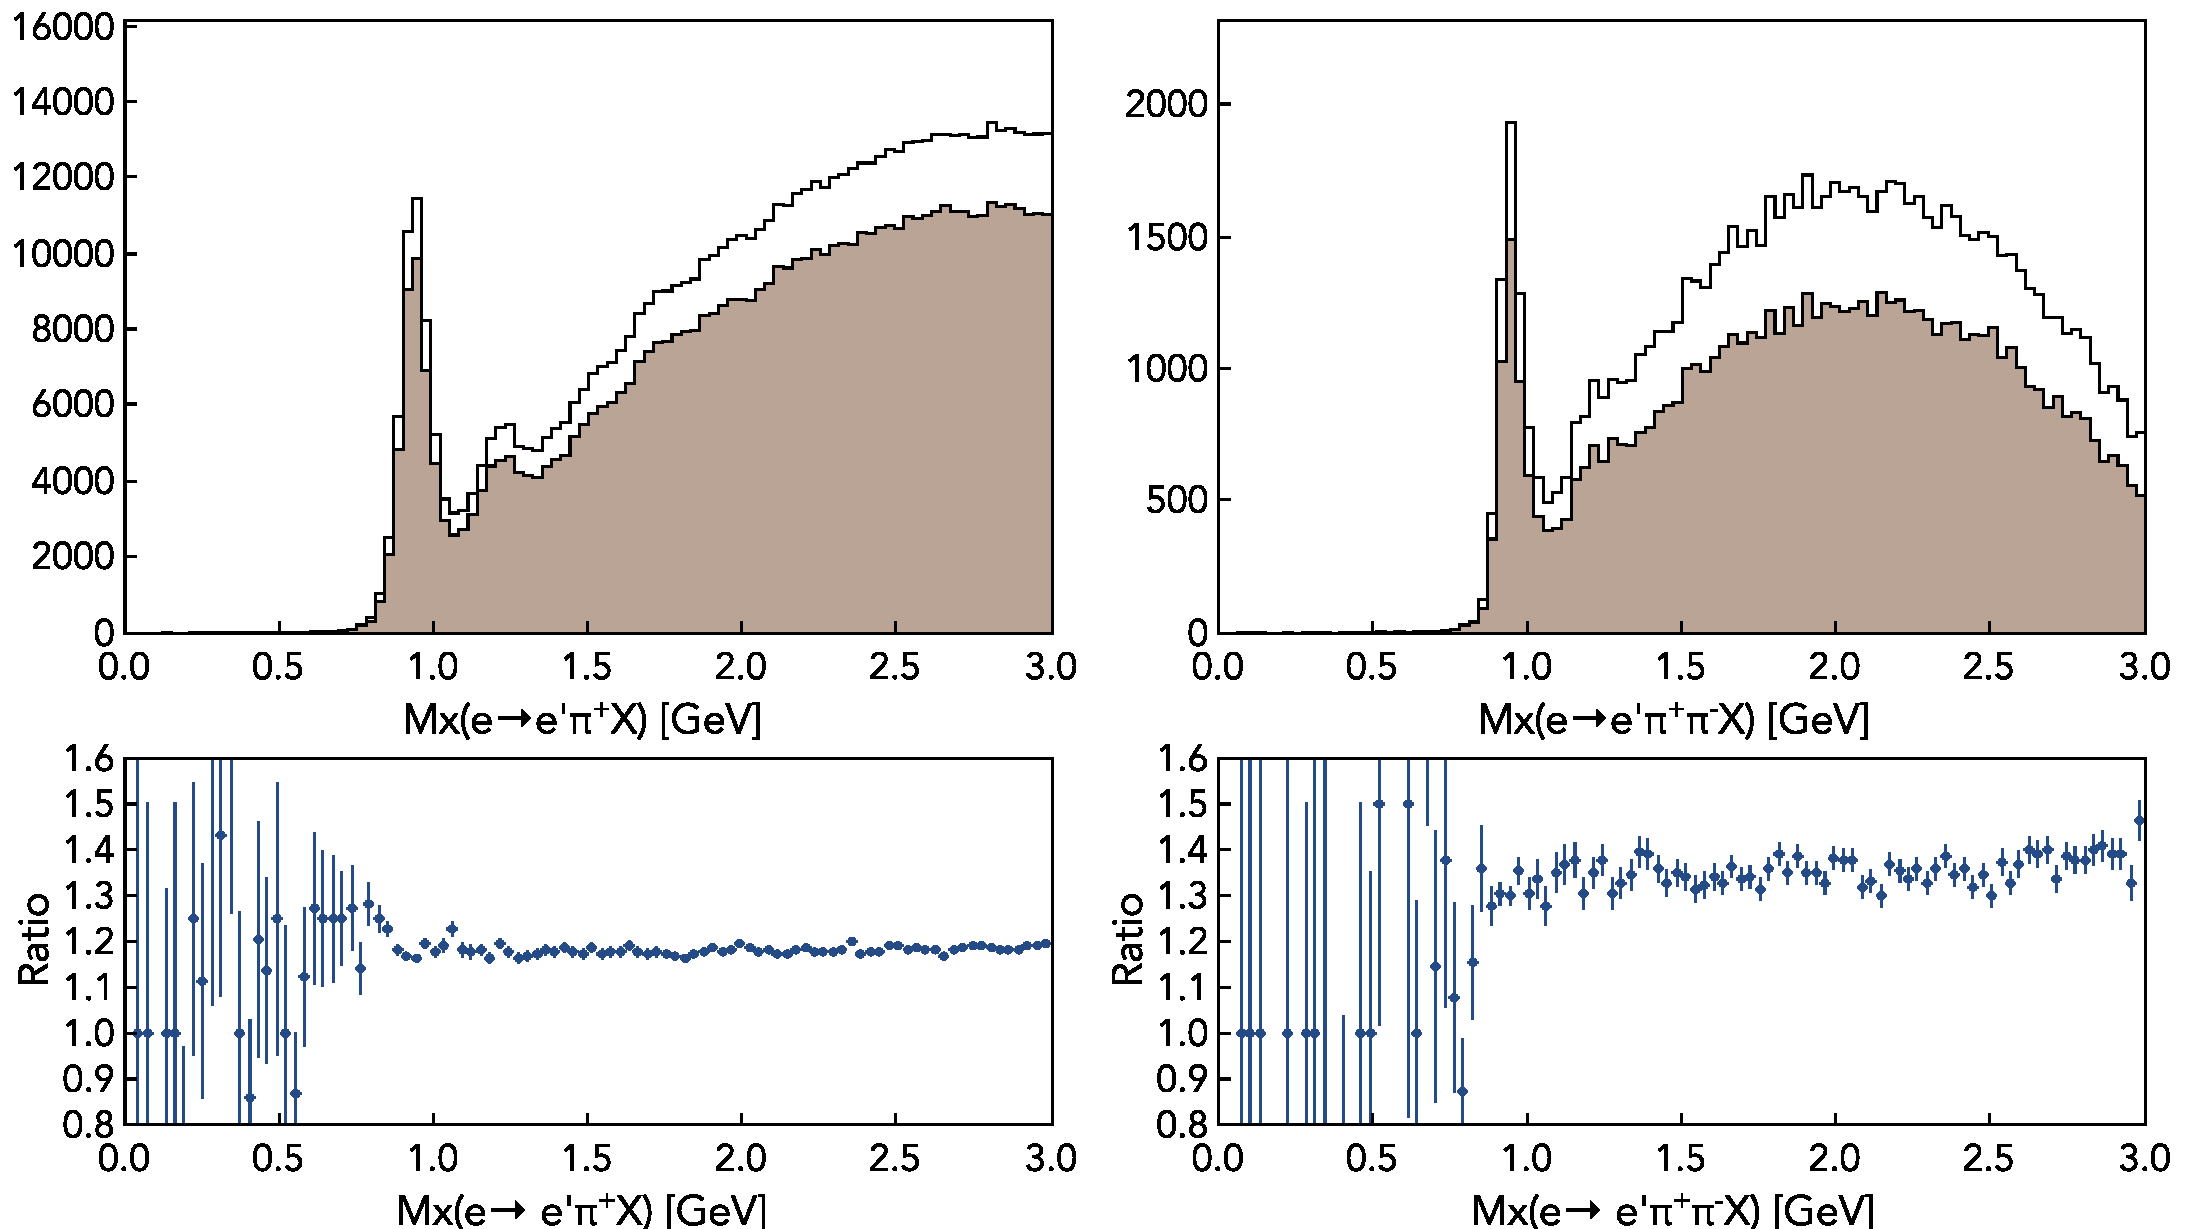
\includegraphics[width=6.0in]{images/physics_scan.pdf}
\caption {Reconstructed missing mass distribution for $H(e,e'\pi^-X)$ and $H(e,e'\pi^+\pi^-X)$ reactions (top row) using the conventional track reconstruction algorithm (filled histogram) and  AI-assisted track reconstruction (black line histogram). The ratios of the two histograms are shown on the bottom row. }
 \label{physics:outcome}
 \end{center}
\end{figure}

The distributions of missing mass for both final state topologies are shown on Figure~\ref{physics:outcome}, where the plots 
on the top row are missing mass of $H(e,e'\pi^-X)$ and $H(e,e'\pi^+\pi^-X)$, where the filled histogram is calculated from 
particles reconstructed by the conventional tracking algorithm, and the histogram with black outline are the same distributions 
calculated from particles that were reconstructed using suggestion from Artificial Intelligence. As can be seen from the figure, 
there is significant increase in the number of events under the missing proton peak (at mass value $0.938~MeV$) for AI assisted
tracking. The ratios of the two histograms (AI-assisted divided by conventional) can be seen on the bottom row of 
Figure~\ref{physics:outcome}. As can be seen from the figure the increase in statistics is uniform over the whole range of the 
missing mass indicating no systematic abnormalities for AI-assisted tracking. The ratio also indicates that there is an increase 
for the number of events under the peak for proton, about $15\%$ for $H(e,e'\pi^-X)$ final state and $30-35\%$ for the $H(e,e'\pi^+\pi^-X)$
final state. Further studies show that improvements in statistics are larger for higher luminosity (incident beam current), which is consistent with our studies of increased efficiency of single particle reconstruction.
%Further studies show that increase in statistics for different final states increase with increase of beam current (luminosity) 
%which is consistent with our studies of increased efficiency of single particle reconstruction. 


\section{Summary}

In this paper we investigated results of analysis of experimental data from CLAS12 detector reconstructed with assistance of Artificial Intelligence
to identify tracks from the hits in drift chambers. This work is based on two neural networks developed to classify track candidates from
given cluster combinations \cite{Gavalian:2020oxg} and to identify missing cluster positions in tracks that do not have complete 6 cluster configuration \cite{Gavalian:2020xmc}. After implementing these networks into the CLAS12 reconstruction workflow, the AI was able to identify ``good'' track candidates 
and pass them to the tracking code to be analyzed parallel to conventional algorithm that chooses``good'' track candidates iteratively considering all possible combinations. 
Our studies showed that AI-assisted tracking performs better than conventional track identification algorithm, and leads to track reconstruction efficiency increase of $15\%$ for nominal experimental running conditions (beam current 45 nA). The AI also performs better with increasing background (i.e. with increased incident beam current) and improves the efficiency loss from $0.44\%$ per nA to $0.24\%$ per nA.
This increased track reconstruction (identification) efficiency directly impacts the outcome of physics analysis where it increases statistics 
for physics reactions for $15\%-35\%$ depending on how many particles are detected in the final state and the topology of the reaction. This has significant implication on experimental running conditions since with increased efficiency the required statistical significance of the experiment can be reached in a shorter time by running at higher beam current (luminosity). Already collected experimental data can be re-processed with the AI-assisted tracking
code which can increase the statistics for analyzed data up to $35\%$. Both, future experiments and already completed ones will benefit 
from this novel development.

Another important outcome of this development was a reduction in data processing times. Since track candidates were identified by AI, there were fewer marginal quality tracks picked to be analyzed and then later dropped due to non-convergence of Kalman filter, leading to tracking code speedup  of $35\%$.

Overall we identified that AI assistance in tracking codes is a good approach, and leads to improvements in code speed and 
efficiency of track reconstruction. Another important aspect of using AI is that is leads to a very small and simple codebase, comprised of composing track candidates and feeding them to the neural networks, and what's also important is that it keeps improving with constant training on new data.
We intend to continue this development in extending the approach to other tracking detectors of the CLAS12, and possibly try to adapt  our approach for other experimental detector setups at Jefferson Lab.

Given the increase in track reconstruction and significant increase in physics statistics for nominal data taking conditions at $45~nA$ we estimated savings of  $\$4.2$M USD. The calculation was done using publicly available budget for operating CEBAF~\cite{CEBAF:oper} adjusted for inflation~\cite{GoogleDotCom}. The calculated budget of ~\$$48$M for all four experimental halls annually means $\approx \$12$M operating budget for CLAS12 experiments, and with $\approx 35\%$ increase in statistics leads to reported savings.




\section{Acknowledgments}

This material is based upon work supported by the U.S. Department of Energy, Office of Science, Office of Nuclear Physics under contract DE-AC05-06OR23177, and
 %This research was sponsored in part from Jefferson Lab grant no. XXX, SURA grant No. CNF-19-04, 
 NSF grant no. CCF-1439079 and the Richard T. Cheng Endowment. The authors would like to thank Raffaella De Vita for help in processing data with CLAS12 reconstruction software. This  work  was  performed  using  the  Turing  and  Wahab computing clusters at Old Dominion University.
 
\newpage
\bibliography{references}
\bibliographystyle{ieeetr}

\end{document}
